\documentclass[thesis,cz]{ctu}

\usepackage{siunitx} %si units
\usepackage{array} % for whole bold rows in tables
\newcolumntype{*}{>{\global\let\currentrowstyle\relax}}
\newcolumntype{^}{>{\currentrowstyle}}
\newcommand{\rowstyle}[1]{\gdef\currentrowstyle{#1}%
  #1\ignorespaces
}

\usepackage{booktabs}
\newcommand{\ra}[1]{\renewcommand{\arraystretch}{#1}}

\usepackage{algpseudocode}
\usepackage{algorithm}
\usepackage{pdfpages}
\usepackage{listings}
% \definecolor{lightpurple}{rgb}{0.8,0.8,1}
\lstset{
    frame=tb,
    numbers=left,
    xleftmargin=2em,
    % numberstyle=\color{red},
    % keywordstyle=\color{blue},
    commentstyle=\color{gray},
    % identifierstyle=\color{black},
    }

% ------------- Colors abbreviations ------------
\def\cbl{\color{blue}}

\ctuTitle{Dual-arm robot perceiving and manipulating soft objects -- use cases}
\ctuAuthor{Tadeáš Lejsek}
\ctuSupervisor{Václav Hlaváč}

\ctuAbstract{
    The thesis explores the possibilities of a various sensoric feedback loops that mimic the human visual and tactile sensing in complex robotic manipulation tasks. I developed four use cases that involve various soft object manipulation tasks with the two-arm \CloPeMa\/ robot such as shooting projectiles from a slingshot, tying an overhand knot, catching a swinging gymnastic pole and regrasping a piece of a rope from one robot arm to the another one. These four use cases will enrich the repository of sensing/manipulation skills in \CloPeMa\/ project and beyond it.
}

\ctuAbstrakt{
    Diplomová práce zkoumá možnosti užití zpětné vazby, která napodobuje lidský zrak a hmat, a to v komplexních robotických manipulačních úlohách. Vypracoval jsem čtyři případové studie, které se zabývají manipulací s~měkkými objekty pomocí dvourukého robotu \CloPeMa\/ jako je střelba z praku, vázání uzlu, chytání kývající se gymnastické tyče zavěšené na gymnastické stuze a přechytávání lana z jedné robotické ruky do druhé. Tyto čtyři případové studie obohatí souhrn manipulačních a percepčních schopností robotu \CloPeMa\/ v rámci projektu \CloPeMa\/ a budou užitečné i po jeho skončení.
}

\renewcommand{\cctuAcknowledgementsBody}{
    I would like to thank my supervisor Václav Hlaváč. His advice given at our regular weekly meetings were highly valuable. His ``top view'' perspective shed new light on many aspects of writing the thesis. My deepest thanks belongs to my direct co-workers at the \CloPeMa\/ project Vladimír Petrík and Libor Wagner. They were always ready to thoroughly answer all of my questions. I have learned a lot from them. I would also like to thank Vladimír Smutný and Pavel Krsek. Vladimír Smutný has been my supervisor even during my high school years when I did several projects for the university. He also guided my pre-diploma work at the \CloPeMa\/ project.

    I would like to thank Marcel who helped me to construct a better slingshot and my friends who participated in making the knot-tying videos. I would also like to thank Tereza Köppelová, a rhythmic gymnast, who showed me how to manipulate the ribbon. I am very thankful to Jéňa who can answer every imaginable question about image processing and who always had time for me and Ondra with whom I could always talk about programming in Python. I would also like to express my gratitude towards my fiancée Bára for her patience. I am very thankful to my parents who always encouraged me to study and even created the conditions that allowed me to study abroad. Last but not least, I would like to thank all of my friends and family members who were always interested in what I am doing and were always eager to see the new videos that I made.

    }


\def\Cplusplus{C\raisebox{0.5ex}{\tiny\textbf{++}}}

\providecommand{\CloPeMa}{\emph{CloPeMa}}


% \includeonly{Src/01intro}
%\includeonly{Src/02SOTA}
% \includeonly{Src/03slingshot}
% \includeonly{Src/04tyer}
% \includeonly{Src/05ribbon}
% \includeonly{Src/regrasping}
% \includeonly{Src/06conclusions}
% \includeonly{Src/implementation}
% \includeonly{Src/07appendix}

\begin{document}
\rhead{Soft objects manipulation and perception} % Shorter title - no overlapping in the heads of the pages

% CTU pages
\ctuTitlePage
\includepdf[pages={1}]{Src/assignment_EN.pdf}
\includepdf[pages={1}]{Src/assignment_CZ.pdf}
\ctuStartPages
\ctuTablesOfContents

\clearpage

% Introduction
\graphicspath{{Img/intro/}}

\section{Introduction}

    \subsection{Motivation}
        Various robots and robotic production lines are used in industry and in other fields on a daily basis. However, in most cases, they are either teleoperated or programmed to repeat a previously learned motion. These robots have mostly a single arm. In case the robots and robotic applications are autonomous, the most widely used sense is the vision.

        However, things are beginning to change. In the article titled ``My boss the Robot'' \cite{bourne13}, David Bourne writes about the future of robots in industry. He points out that the time when robots operated in isolated cells repeating a certain motion over and over might soon change. Since humans and robots are best at different tasks (e.g. complex manipulation and precise welding), it would be very smart to efficiently combine their skills. For that reason, robots and humans would have to work side by side collaborating on a given task. In these cases, the robot has to use a variety of sensors to sense its human colleague. And this is just one of the points where different kinds of feedback other than visual come into play.

        I personally find it very exciting to develop a new sense for the robots -- the tactile sensing that mimics the human sense of touch. Since the time the visual feedback has been introduced, the robots have been able to accomplish many more tasks. The same promises the introduction of the tactile feedback. It involves tasks ranging from robotic surgeons up to automated manipulation with clothes.

        The \CloPeMa\/ project aims at advancing the state-of-the-art in such areas. My work is focused at using the tactile, kinesthetic and visual feedback in different tasks such as automated knot-tying and demonstrating their functionality.

    \subsection{\CloPeMa\/ project context}

        The project context description is taken from a report that I created in the previous semester~\cite{PreDiplomaLejsekHlavac}.


        \CloPeMa\/ is a three year European Commission funded research project in the Framework Program~7, which advances the state of the art in the autonomous perception and manipulation of soft materials such as fabrics, textiles and garments. \CloPeMa\/ runs  between February 2012 and January 2015. There are five partners cooperating in the project (from Greece, Italy, Scotland and two partners from the Czech Republic). \CloPeMa\/ test-bed utilizes a dual-arm robot based on the industrial welding arm Motoman 1400. \CloPeMa\/ modules are integrated on top of Robotic Operating System (ROS).

        \begin{figure}[h]
        \centering
        \begin{tabular}{cc}
        \includegraphics[width=0.57\textwidth]{tshirt02.png}
        %
        &
        %
        \includegraphics[width=0.39\textwidth]{CloPeMaForceTorqueSensorSmAnnotatedCrop}
        \end{tabular}
        \caption{Left: \CloPeMa\/ project dual-arm robot manipulating a T-shirt. Right: The force /~torque sensor Mini45 ATI mounted on \CloPeMa\/ robot.}
        \label{fig:CloPeMaRobot-and-FTsensor}
        \end{figure}

        In the run of \CloPeMa\/ project, a force compliant 13-DOF dual-arm robot formed by two industrial arms Motoman 1400 has been implemented and equipped with two off-the-shelf force/torque sensors (ATI-Mini45) in between the last joint and the gripper, see Figure~\ref{fig:CloPeMaRobot-and-FTsensor}, right side. Each arm hosts a custom build sensorized gripper with actively controlled compliance capable of rubbing motions of the fingers.

        \CloPeMa\/ test-bed is rich in sensors. The sensor setup is formed by: the Kinect-like sensor ASUS Xtion on both forearms, the precise optical stereo on the central pole (formed by two SLR Nikon cameras); the gripper hosts a photometric stereo camera in the palm of the gripper, and is equipped with the 16-elements capacitive tactile sensor in the gripper finger. The view of the \CloPeMa\/ system folding a T-shirt is in Figure~\ref{fig:CloPeMaRobot-and-FTsensor}, left side.

        \begin{figure}[h]
        \centering
        \begin{tabular}{cc}
        \includegraphics[width=0.48\textwidth]{CloPeMaGripperEntireView1Sm}
        %
        &
        %
        \includegraphics[width=0.48\textwidth]{CloPeMaGripperTactileSensorSm}
        \end{tabular}
        \caption{Left: The \CloPeMa\/ hand with variable stiffness and tactile sensor. Right: Detail of the hand tip with the tactile sensor.}
        \label{fig:CloPeMaHand}
        \end{figure}

        \begin{figure}[h]
        \centering
        \includegraphics[width=0.5\textwidth]{CloPeMaGripperHydraulicsSm}
        \caption{Gripper hydraulics controller box.}
        \label{fig:CloPeMaHandHydraulics}
        \end{figure}

        The gripper has a controllable impedance by involving hydraulics and air bubbles injected into the hydraulic oil. The hydraulic actuator is visible in Figure~\ref{fig:CloPeMaHand} left side. The gripper has a capacitive 16 texels tactile sensor in the upper finger in Figure~\ref{fig:CloPeMaHand}, right side. The source of hydraulic energy is placed on the arm of the robot farther from the gripper, see Figure~\ref{fig:CloPeMaHandHydraulics}.

        \CloPeMa\/ project inheritance is also in established integration procedures on top of Robotic Operating System (ROS), software design practices in  \Cplusplus\/ and Python, established project management support using Redmine tool, etc.

    \subsection{Goals of the thesis}
    Based on the given thesis assignment, I specified my own assignment for each of the given tasks more in detail.

        \subsubsection{Slingshot}
        The aim is to explore the possibilities of the compliant motion and the force feedback. The force sensor will be used mainly. The goal is to design an automated slingshot and to find out whether an automated procedure for hitting a standing target can be developed. I came up with the following scenario:
            \begin{enumerate}
                \item Develop an automated slingshot.
%
                \begin{enumerate}
                    \item Initial position: one robot arm holds the slingshot, the other arm holds the projectile.
                    \item Load the projectile.
                    \item Stretch the elastic string of the slingshot so that it exerts the given force on the projectile.
                    \item Shoot the projectile at a given shooting angle.
                \end{enumerate}
%
                \item Compare the theoretical analysis of the shooting (i.e. which point should be hit by the projectile based on its initial speed, shooting angle etc.) with the actual experiments.
            \end{enumerate}


        \subsubsection{Knot-tying}
            The goal is to tie an overhand knot in the air using the two-arm robot. Various sensors might be used, for instance Xtion kinect and the force sensor.

            I came up with the following solution to the knot tying problem. The robot is already holding the rope in both grippers at the beginning of the proposed procedure.
%
            \begin{enumerate}
                \item Wrap the rope around the left arm in a way that a loop is created.
                \item Release the rope end with the right arm and move the right arm away.
                \item Turn the left arm so that the left camera sees the loop and the rope end.
                \item Detect the rope end and catch it with the right arm.
                \item Tighten the knot using both arms.
            \end{enumerate}

        \subsubsection{Ribbon manipulation}
            I chose a manipulation with the rhythmic gymnastic ribbon and pole to be the third task. The aim of it is to mimic a few capabilities of a human rhythmic gymnast. I am especially interested in tasks that involve dynamics and in investigating the capabilities of the robot grippers.

            I proposed a following scenario. At the beginning, the robot is holding the pole hanging on a ribbon in its left gripper.
%
            \begin{enumerate}
                \item Swing the left arm in a way that the pole and ribbon start to swing as well.
                \item Catch the pole with the right gripper using one of the many sensors that are present in the gripper.
                \item Make sure the gripper holds the pole well (and that it was caught) and release the ribbon with the left arm.
                \item Perform a few fast moves with the right arm so that the ribbon forms a certain shape, which is nice to watch.
           \end{enumerate}

        \subsubsection{Regrasping a rope}
            The last use case deals with the regrasping of a piece of a rope from one gripper to the other one. The light or proximity sensor should be used to detect the presence of the rope in the gripper. This section should demonstrate that it is indeed possible to swap the functions of both robot arms.

            The proposed scenario is the following. The left gripper holds one end of the rope. The right gripper is open and is positioned towards the left gripper.
%
            \begin{enumerate}
                \item The left arm starts to move towards the right gripper.
                \item When the presence of the rope is detected inside the right gripper, the motion of the left arm is stopped.
                \item The right gripper closes, thus holding the other end of the rope.
                \item The left gripper opens and releases the rope.
                \item The left arm moves back and the functions of both arms are swapped.
                \item The whole procedure is repeated again. The right arm now moves towards the left one that catches the rope.
            \end{enumerate}



    \subsection{Thesis organization and naming robot arms}
        The thesis is organized into seven bigger sections -- one section describing the state-of-the-art, four sections for each of the given tasks, one section that describes the implementation and the last section provides conclusions. Each task description contains all the related information -- assignment, analysis, experiments and discussion.

        The two arms of the \CloPeMa\/ robot are called \textit{R1} and \textit{R2}. \textit{R1} is the right arm and \textit{R2} is the left arm from the view of the robot. This naming convention is then used further on in the text.

\clearpage 

% State-of-the-art
\graphicspath{{Img/SOTA/}}

\chapter{State-of-the-art}

    \section{General}
A tactile feedback is useful for perceiving and manipulating soft objects. Its usage dates back to at least 1987 when Stephen Buckley, USA published his PhD on planning and teaching compliant motion strategies \cite{Buckley1987Insertion}. He was for instance interested in scenarios, in which a robot holds a T-shaped piece that has to be inserted into a corresponding hole. He worked with a robotic arm capable of Cartesian motions, but not rotations. The robot arm was modeled as a damped spring. A method how to teach the robot the wanted motions was developed.

Another example of the usage of the tactile feedback is a task where a human guides a robotic arm by hand. It was implemented at Weiss Robotics, Germany \cite{Weissrobotics} (see Figure~\ref{fig:CompliantMotion}, left side). Such scenario might be very useful in industry and other areas. A human can teach the robot a certain motion quickly without the need to specifically program it.

        \begin{figure}[h]
            \centering
            \begin{tabular}{cc}
            \includegraphics[height=0.3\textwidth]{WeissRobotics.png}
            %
            &
            %
            \includegraphics[height=0.3\textwidth]{CompliantMotion.png}
            \end{tabular}
            \caption{Left: Manually guiding the robot arm by hand at Weiss Robotics. Right: Manually guiding the robot arm by hand at \CloPeMa\/.}
            \label{fig:CompliantMotion}
        \end{figure}

        In case the force sensor is not placed at the tip of the robot arm, the weight of everything that is placed below the force sensor has to be subtracted in order to get a correct force/torque measurement. This procedure of separating the weight caused by inertia from the influences of the environment (e.g. a human hand) is described in \cite{2006Kroger6DForceSensorFusionIROS}. The same procedure is used in case of the \CloPeMa\/ robot, where force/torque sensors are placed in both wrists \cite{KubesForceSensor}. Together with my college Jan Kubeš, we implemented the manual guidance of the robot arm at the \CloPeMa\/ robot \cite{PreDiplomaLejsekHlavac}. The experiment was recorded on video \cite{ClopemaCompliantMotionKubesLejsek} and is shown in Figure~\ref{fig:CompliantMotion}, right side.

        Another field where a tactile/haptic feedback is used is surgery. A robotic simulator using virtual force feedback was designed at Intelligent Robotics Institute, China \cite{syed2011maxillofacial}. A human surgeon should already be well trained when performing a complicated maxillofacial surgery. For this reason, a platform featuring a 6-DOF robotic arm, haptic and visual feedback was developed to help to train young surgeons.

        A field in which the tactile feedback would be beneficial is the autonomous garment folding (see Figure~\ref{fig:ClopemaFoldingTShirt}). The present solution developed in the course of the \CloPeMa\/ project predominantly utilizes the visual feedback. The usage of the tactile feedback in \CloPeMa\/ testbed is planned for the future~\cite{stria2014garment}.

        \begin{figure}[h]
        \includegraphics[width=0.4\textwidth]{ClopemaFoldingTShirt.png}
        \centering
        \caption{The \CloPeMa\/ robot folding a T-shirt.}
        \label{fig:ClopemaFoldingTShirt}
        \end{figure}

        A compliant robot arm can also be made cheaply. The reduction of price was achieved through several choices such as not using an expensive robot head and using stepper motors \cite{quigley2011low}. The arm is capable of playing chess (via teleoperation) and making pancakes (see Figure~\ref{fig:RobotPancakes}).

        \begin{figure}[h]
        \includegraphics[width=0.4\textwidth]{RobotPancakes.png}
        \centering
        \caption{The 7-DOF compliant robot arm making pancakes.}
        \label{fig:RobotPancakes}
        \end{figure}

    \section{Slingshot}
        As far as I know, nobody else has used a two-arm robot for experimenting with a slingshot.
        However, other scenarios have been explored.

        One example is the ``David and Goliath'' slingshot (see Figure~\ref{fig:DavidsSlingshot}). The projectile (a stone) is thrown using a rotating slingshot. The ``robotic'' realization was implemented at University of Pisa, Italy, 2011. It can be seen in the video \cite{DavidLikeSlingshot}.

        \begin{figure}[h]
        \includegraphics[width=0.5\textwidth]{DavidsSlingshot.png}
        \centering
        \caption{The principle of the rotating slingshot.}
        \label{fig:DavidsSlingshot}
        \end{figure}


        Another example is the ``Trebuchet'' scenario. This principle was used in siege machines in antiquity. Its realization in robotics is shown in \cite{Trebuchet} made by Lake Area Technical Institute (USA) students.

        Finally, another scenario uses the principle of two fast rotating disk. When a projectile (in this case a ball) gets in between them, it is shot forwards. The realization was done by Team 5353, Fremont, USA \cite{TwoRotatingDisks}.

    \section{Knot-tying}

        \begin{figure}[h]
        \includegraphics[width=0.5\textwidth]{PR2Knot.png}
        \centering
        \caption{The PR2 robot tightening a knot at UC Berkeley.}
        \label{fig:PR2Knot}
        \end{figure}

        Knot tying was  done for instance in UC Berkeley, USA. They used the Willow Garage PR2 robot and their working scenario was the following. A rope was lying on the table, the robot sensed it, planed how to tie the knot and finally made a simple overhand knot while the rope was still lying on the table (see Figure~\ref{fig:PR2Knot}). The whole process involves only one arm of the two-arm robot. Both arms were used only at the end of the whole procedure to tighten the knot. The rope was segmented based on its color. The robot was taught by a human guidance beforehand~\cite{UCBerkeleyOverhandKnotArticle}. The whole procedure is shown in the video~\cite{UCBerkeleyOverhandKnotVideo}.

        Another working scenario is to entirely omit the need to regrasp the string by using so called fixtures (knot boxes). Such work was done at Darthmouth College, Hannover, Germany \cite{FixtureKnotTying}.

        A great benefit from autonomous knot tying would be in Minimally Invasive Surgery (MIS).  Long Short-Term Memory neural networks were trained using supervised learning to autonomously tie suture knots on a surgical robot (see Figure~\ref{fig:SutureKnot}) \cite{SutureKnotTying}. This work was done in cooperation of Technical University Munich, Germany and Istituto Dalle Molle di Studi sull’Intelligenza Artificiale (IDSIA), Switzerland.

        \begin{figure}
        \includegraphics[width=0.35\textwidth]{SutureKnot2.png}
        \centering
        \caption{The suture knot.}
        \label{fig:SutureKnot}
        \end{figure}


    \section{Ribbon manipulation}
        To the best of my knowledge, nobody has used a two-arm robot for a manipulation with a modern gymnastic ribbon.

        \begin{figure}[h]
        \includegraphics[width=0.4\textwidth]{Justine.png}
        \centering
        \caption{The Rollin' Justin Robot catching a ball.}
        \label{fig:Justine}
        \end{figure}

        However, scenarios where a robotic arm catches a flying object, e.g. a ball are being researched as this setup is used as a benchmark for key robotic technologies. An example is the work done at DLR Institute for Planetary Research, Germany. A high speed 7-DOF robotic arm is used for ball catching. The whole system has to meet hard real-time operation deadlines and thus a lot of computational power is needed (a cluster with 32 CPU cores). The catch rate is reported to be > 80\%, the visual sensing being the weakest point of the whole system \cite{FastBallCatching}. The arm is a part of Rollin' Justin Robot \cite{FastBallCatchingVideo} (see Figure~\ref{fig:Justine}).

        Fast and repeatable motions are needed in the industry. The example of that is a demo made by ABB robotics \cite{CanChallengeVideo}.

    \section{Grasping objects}
        Robotic object grasping is a complex topic. It was studied for instance at Carnegie Mellon University, Pennsylvania, USA \cite{kazemi2012robust}. The authors showed in 2011 that in order to develop a robust grasping of relatively small objects such as pens, screwdriver, cellphones and hammers, the robotic fingers should come in touch and make use of the supporting surface.

        A Mobile Manipulator that is able to autonomously fetch an object lying on a flat surface was developed in 2010 at Georgia Institute of Technology \cite{jain2010assistive}. The aim is to improve the everyday life of elderly, injured or disabled people (see Figure~\ref{fig:AssistiveManipulator}). A tilting laser range finder is used to acquire 3D point cloud data around the surroundings of the object to be fetched.

        \begin{figure}[h]
        \includegraphics[width=0.4\textwidth]{AssistiveManipulator.jpg}
        \centering
        \caption{The mobile manipulator, EL-E, delivering an object to a patient.}
        \label{fig:AssistiveManipulator}
        \end{figure}

\clearpage 

% Slingshot
\graphicspath{{Img/slingshot/}}

\chapter{Slingshot}

\section{Assignment}
The work performed in this thesis follows closely the work, which I did in the subject called ``Individual project''~\cite{PreDiplomaLejsekHlavac}, where I focused on exploring the possibilities of a robotic slingshot. Here I continue with developing a fully automated slingshot.
	
The goal is to implement the following shooting procedure. The right arm holds the projectile and the slingshot is attached to the left one.
%
		\begin{enumerate}\itemsep0pt
		    \item Load the projectile. Use force feedback to determine that the elastic string has been touched.
		    \item Stretch the elastic string of the slingshot by moving the attached projectile using the right arm. Stop when the exerted force exceeds a predefined threshold.
		    \item Adjust the shooting angle by the left arm. Shoot the projectile.
		\end{enumerate}	


\section{Analysis}

\subsection{Attaching the slingshot to the robot arm}		

\begin{figure}[h]
\includegraphics[width=0.35\textwidth]{slingshot_traditionalAdj.png}
\centering
\caption{The traditional slingshot.}
\label{fig:traditional slingshot}
\end{figure}	

There is one major difference to my previous work \cite{PreDiplomaLejsekHlavac}, though. The gripper of the \CloPeMa\/ robot has been changed in the meantime. It is not possible to attach the elastic string directly to the gripper, because the projectile could damage the sensors in the new gripper seriously. Therefore, I had go back to the original idea of the ``traditional slingshot'' (see Figure~\ref{fig:traditional slingshot}).

The slingshot cannot be held in the gripper. If just a small force is exerted on the elastic string, the gripper is not able to hold the slingshot anymore. Thus, the slingshot has to be attached directly to the robotic arm (see Figure~\ref{fig:attached slingshot}). I did it using velcro. It is then easy to attach and remove the slingshot within a few moments. The only disadvantage is that the slingshot might move slightly, if a high force is exerted on it. However, to completely avoid this problem, the slingshot would have to be designed differently.

			\begin{figure}[h]
			\includegraphics[width=0.5\textwidth]{attached_slingshotAdj.png}			
			\centering
			\caption{The attached slingshot.}
			\label{fig:attached slingshot}
			\end{figure}		
	
	
		\subsection{Workflow of the shooting procedure} \label{subsec: traditional workflow}
The procedure for shooting projectiles using the slingshot is described by the finite state machine that is shown in Figure~\ref{fig: slingshot workflow}.
			
			\begin{figure}
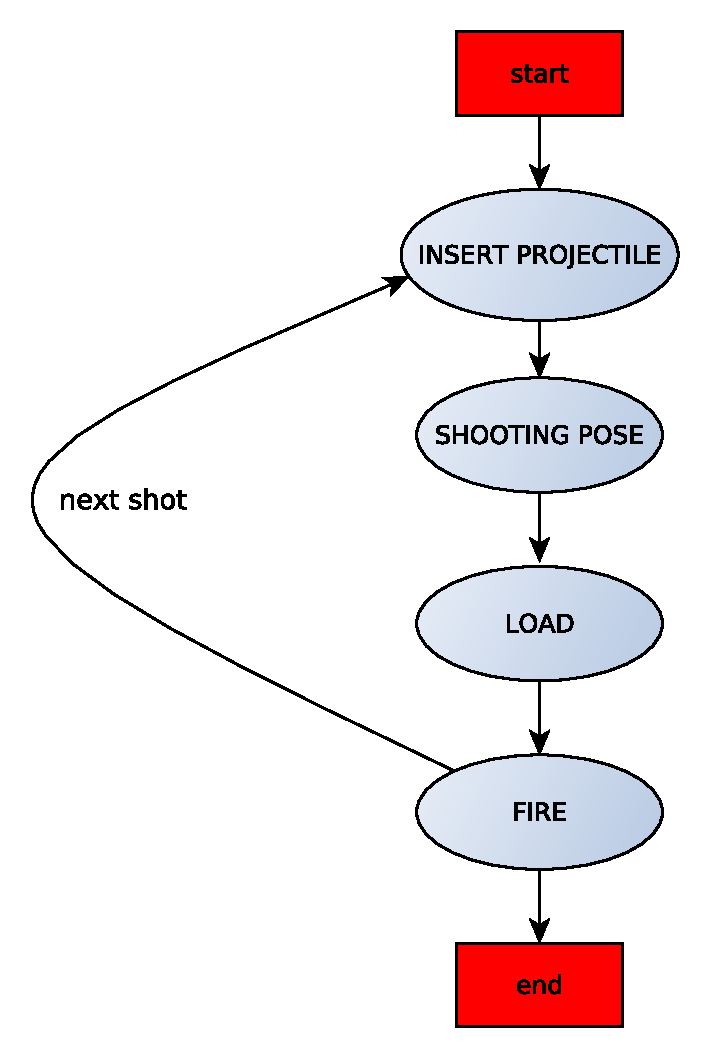
\includegraphics[height=0.5\textheight]{SlingshotStateMachine.pdf}						\centering
			\caption{Slingshot workflow.}
			\label{fig: slingshot workflow}
			\end{figure}


			\begin{figure}
			\includegraphics[width=0.25\textheight]{slingshot_process.png}			
			\centering
			\caption{Slingshot process diagram -- the top view.}
			\label{fig: slingshot process}
			\end{figure}		
			
			The flow chart connected with the shooting process is shown in Figure~\ref{fig: slingshot process}.
				
			\paragraph{Insert the projectile}~\\
				\indent The projectile is inserted into the gripper manually.
				
				A little trick is used to simplify this procedure for the operator. Normally, the operator presses a button to close the gripper. But when the operator enters the safety cage with the robot to insert the projectile, it is hard to reach the keyboard. Therefore, the gripper closes, when the force exerted on it exceeds a certain threshold. Thus, no keyboard is needed to close the gripper after the projectile has been inserted (see Figure~\ref{fig:ProjectileInsertion}).

				\begin{figure}
				\includegraphics[width=0.5\textheight]{ProjectileInsertionAdj.png}			
				\centering
				\caption{Inserting the projectile.}
				\label{fig:ProjectileInsertion}
				\end{figure}

				
			\paragraph{Shooting position (A)}~\\
				\indent The right arm of the robot moves next to the slingshot.
				
			\paragraph{Load (B, C)}~\\
				\indent The right arm holding the projectile moves towards the elastic string. The movement stops, when the projectile touches the string (B). It is detected by the force sensor in the right arm. When the force exceeds a certain threshold force $F_B$, the movement is stopped. The arm then moves a bit back (C).
				
			\paragraph{Fire (D)}~\\
				\indent The right arm moves backwards (D) until the desired force $ F_D$ is reached. Then the gripper opens and the projectile is released.

		\subsection{Force/torque sensor}
			In order to implement projectile insertion, loading and firing, a force feedback is needed. There are two ATI Mini 45 force sensors placed in the wrist of each arm. The force sensor measures the force and torque simultaneously in three axes. Thus, it provides $F_{x, y, z}$ and $T_{x,y,z}$ at the maximum frequency of \SI{7,000}{Hz}. After the filtration of the outside disturbances (such as trams and light disturbances) and subtracting the weight of the gripper, the sensor provides the meaningful data at the frequency of \SI{12.5}{Hz}~\cite{KubesForceSensor}. I use the force measurements only.
	
	
	\section{Experimental setting}

		\subsection{Shooting scene}
		
			Figure~\ref{fig:shooting setting} shows two settings of the shooting with the slingshot. The left diagram shows the horizontal shooting, the right one the shooting upwards. The shooting parameters were $z_0 = $ \SI{1.9}{m}, $ d = $ \SI{1.85}{m}.
			
			\begin{figure}[h]
			\centering
			\begin{tabular}{cc}
			\includegraphics[width=0.48\textwidth]{horizontal.png}
			%
			&
			%
			\includegraphics[width=0.48\textwidth]{askew.png}
			\end{tabular}
			\caption{Left: Shooting horizontally. Right: Shooting upwards.}
			\label{fig:shooting setting}
			\end{figure}
			
	
		\subsection{Projectile}
			A bent piece of wire was chosen to be the projectile (see Figure~\ref{fig: projectile}) for the following reasons. Firstly, the gripper can hold it, even if a high force is exerted on it. Secondly, it is light and finally, because it has a low air resistance.

			\begin{figure}[h]
			\includegraphics[width=0.5\textwidth]{bulletAdj.png}			
			\centering
			\caption{The projectile.}
			\label{fig: projectile}
			\end{figure}
			
			The weight of the projectile $m$ was measured to be in the range~1 to~\SI{2}{g}.
			
			When the projectile is shot, it leaves the slingshot with the initial velocity $ v_0$. Its magnitude is given by Equation~\eqref{eq: v0} and is derived assuming that the potential energy of the elastic string $ E_p$ is fully converted into the kinetic energy of the projectile $ E_k$. The diagram connected to shooting the projectile is shown in Figure~\ref{fig: shooting projectile}.
			
\begin{align}
E_p & = E_k \\[1ex]
%
\frac{1}{2}F \Delta x & = \frac{1}{2} m v_0^2 \nonumber \\[1ex]
%
v_0 & = \sqrt{\frac{F \Delta x}{m}}
\label{eq: v0}
\end{align}	
			
			The distance $ \Delta x$ is measured from the moment the force sensor detects a non-zero force until the moment when the desired force is reached.
			
			\begin{figure}
			\includegraphics[width=0.35\textwidth]{force.png}			
			\centering
			\caption{Shooting the projectile.}
			\label{fig: shooting projectile}
			\end{figure}

	\section{Implementation}

		\subsection{Force feedback}	

			A key task is to use the force feedback. Force thresholds $F_B$ and $F_D$ are used to detect hitting the elastic string (B) and to detect reaching the firing position, respectively. In addition, the force threshold $F_{D0}$ is used to detect that the elastic string starts to be stretched. This information is used to compute the distance $\Delta x$.

		\subsection{Traditional slingshot} \label{sec: implementation of slingshot 1.0}
		The slingshot script version 1.0 is called the shooter. The usage of the force feedback is implemented incrementally. It means that the arm moves a certain distance (e.g. \SI{1}{cm}) and then the force data is retrieved and checked whether it exceeds a certain force threshold. If not, another step is performed and the whole procedure is repeated. It results in a bit jerky movement of the robotic arm.
	
	\section{Mathematical description}
	
		The assumptions for the following mathematical description are the following.
%		
\begin{enumerate}\itemsep0pt
			\item The projectile is considered to be a point mass.
			\item The projectile has no air resistance.
			\item It is assumed that the motion takes place in a homogeneous gravitational field.			
\end{enumerate}	
		
		\subsection{Shooting horizontally}			
			
			Using the assumptions 1 and 2, the kinematics of the horizontal shooting is given by the two following Equations \eqref{eq: horizontal x} and \eqref{eq: horizontal z}. It is connected with the left side of Figure~\ref{fig:shooting setting}.
		
			\begin{equation} \label{eq: horizontal x}
				x = v_0 t
			\end{equation}
			\begin{equation} \label{eq: horizontal z}
				z = z_0 - \frac{1}{2} g t^2
			\end{equation}
			
			The time $ t_1$, in which the projectile hits the point $P_1 =  [x_1, z_1] = [d, z_1]$ on the opposite wall, is given by:
			
			\begin{equation}
				t_1 = \frac{d}{v_0}
			\end{equation}
			
			The z-coordinate $ z_1$ is then:
			
			\begin{equation} \label{eq: horizontal z1}
				z_1 = z_0 - \frac{1}{2}g t_1^2 = z_0 - \frac{g d^2}{2 v_0^2}
			\end{equation}
		
		\subsection{Shooting upwards}
		
			The setting of the shooting upwards corresponds to the right side of the Figure~\ref{fig:shooting setting}. Its kinematics is given by Equations \eqref{eq: upwards x} and \eqref{eq: upwards z}.
			
			\begin{align}
				x = v_0 \, t \, \cos \alpha \label{eq: upwards x} \\
				z = z_0 + v_0 \, t \, \sin \alpha - \frac{1}{2}g t^2 \label{eq: upwards z}
			\end{align}
			
			The time $ t_1$, in which the projectile hits the point $P_1 =  [d, z_1]$ on the opposite wall, is given by:
			
			\begin{equation}
				t_1 = \frac{d}{v_0 \, \cos \alpha}
			\end{equation}
			
			The z-coordinate $ z_1$ is then:
			
			\begin{equation} \label{eq: upwards z1}
				z_1 = z_0 + v_0 \, t_1 \, \sin \alpha - \frac{1}{2}g t_1^2 = z_0 + d \, \tan \alpha - \frac{1}{2}g t_1^2
			\end{equation}
			

				
	\section{Experiments with the traditional slingshot}
	
		\begin{figure}[h]
		\centering
		\begin{tabular}{cc}
		\includegraphics[height=111px]{string_horizontal.png}
		%
		&
		%
		\includegraphics[height=111px]{string_upwards.png}
		\end{tabular}
		\caption{Left: Straight elastic string ($ \alpha = 0$). Right: Bent elastic string ($ \alpha > 0$).}
		\label{fig:shooting string}
		\end{figure}		
	
		\subsection{Shooting horizontally}
			The first shooting experiment was conducted with a completely straight tightened elastic string. Thus, $ \alpha = 0$ and the projectile was shot horizontally. Figure~\ref{fig:shooting string}	left shows the side view of the slingshot.
			
			The projectile was shot in the following setting: $ F_1 = $ \SI{4.4}{N}, $ \Delta x = $ \SI{0.05}{m}. The shot hit the wall at the height $ z_1 = $ \SI{0.5}{m}. Thus, the initial velocity $ v_{01d}$ was \SI{10.49}{ms^{-1}} according to Equation~\eqref{eq: v0}.
			
			It is possible to estimate the initial velocity from the point $ P_1 = [d, z_1]$. Using Equations~\eqref{eq: horizontal x} and \eqref{eq: horizontal z}, we obtain:
			
			\begin{equation}
				v_0 = d \: \sqrt{\frac{g}{2(z_0 - z_1)}}
			\end{equation}
			
			In our case, $ v_{01k} = $ \SI{3.46}{ms^{-1}}.
			
			Thus, there is a substantial difference (roughly three times) between the initial velocity $v_{01d}$ (calculation based on the parameters of the elastic string and its dynamics) and the initial velocity $v_{01k}$ (calculation based on the kinematics of the horizontal shooting). This suggests that the theoretical model does not fit with the reality.
			
		\subsection{Shooting upwards}
			To make the shooting look as shooting and not as a ``piece of wire falling down'', $ \alpha$ was set to be higher than zero. I accomplished this by moving the elastic string a bit to the side (see Figure~\ref{fig:shooting setting} right). Parameters $ a = $ \SI{6}{cm} and $ c = $ \SI{6.1}{cm} yield:
			\begin{equation}
				\alpha = \arccos \left(\frac{a}{c} \right) \approx 10^{o}
			\end{equation}
			
			Given $ F_1$ and $ \Delta x$, the z-coordinate $ z_1$ of the point $ P_1$ can be computed using Equation~\eqref{eq: upwards z1}). However, the theoretical calculation is very sensitive to the change in $ \alpha$ and $ \Delta x$. Table \ref{table: change in alpha} shows how the change in $ \alpha$ (given $\Delta x = $ \SI{7}{cm} and $F_1 = $ \SI{4.8}{N}) influences $z_1$. Table \ref{table: change in dx} shows how the change in $ \Delta x$ (given $ \alpha = 10^{o}$ and $F_1 = $ \SI{4.8}{N}) influences $z_1$.

			\begin{table}\centering
			\ra{1.3}
			\begin{tabular}{@{}cc@{}}\toprule
			$\alpha$ [$^{o}$] & $ z_1$ [\SI{}{cm}] \\ \midrule
			
			5  & 105 \\
			10 & 120 \\
			15 & 132 \\
			20 & 144 \\
			 \bottomrule
			\end{tabular}
			\caption{Change in $\alpha$.}
			\label{table: change in alpha}
			\end{table}
			
			\begin{table}\centering
			\ra{1.3}
			\begin{tabular}{@{}cc@{}}\toprule
			$\Delta x$ [\SI{}{cm}] & $ z_1$ [\SI{}{cm}] \\ \midrule
			
			5 & 78 \\
			6 & 102 \\
			7 & 120 \\
			8 & 132 \\
			9 & 142 \\
			\bottomrule
			\end{tabular}
			\caption{Change in $ \Delta x$.}
			\label{table: change in dx}
			\end{table}
			
			The actual $ \Delta x_1$ and $F_1$  were measured to be $\Delta x_{1m} = $ \SI{5}{cm} and $F_{1m} = $ \SI{4.8}{N}. The shots were oscillating around the height $z_{1m} =$ \SI{150}{cm}.
			
			The theoretical $z_{1t}$ corresponding to the measured $\Delta x_{1m}$ and $F_{1m}$ is $z_{1t} = $ \SI{78}{cm}.
			
			To achieve the measured $z_{1m}$ given $F_{1m}$, $ \alpha$ and $\Delta x$ would have to be e.g. $\alpha_t = $ \SI{25}{\degree} and $\Delta x_{1t} = $ \SI{7}{cm}.
			
			A video called \textit{TraditionalSlingshot.mpg} was taken that shows the whole shooting procedure. It can be found on the attached CD.

	
	\section{Experiments with the flat slingshot}
		The previous experiments with the traditional slingshot had one problem. It was not possible to attach the traditional slingshot to the robot, so that it does not move while shooting. This behavior means that it is not possible to measure the shooting angle $\alpha$ properly and thus it is not possible to compare the measured results with the theoretical analysis.

		Therefore, a new slingshot model was introduced -- ``flat slingshot'' (see Figure~\ref{fig:flat slingshot}). It is made from plank wood. Its sides are flat and thus it is possible to attach it tightly to the arm of the robot.

		\begin{figure}
		\includegraphics[width=0.5\textwidth]{attached_flat_slingshot.png}			
		\centering
		\caption{The flat slingshot.}
		\label{fig:flat slingshot}
		\end{figure}

		\subsection{Changes to the traditional slingshot}
			The shooting procedure was changed a bit as well compared to the original one, see Section~\ref{subsec: traditional workflow}. The insertion of the projectile and moving to the shooting position was flipped.

			Secondly, the implementation of loading and firing was changed, see Section~\ref{sec: implementation of slingshot 1.0}, as well. The motion of the robotic arm is no longer jerky as it was before. Now the arm does not move incrementally in \SI{1}{cm} steps and does not check the measured force value only after one step was performed.  The smooth movement was achieved. However, the speed of the robot is slowed down ten times and the movement and force checking for threshold values are performed simultaneously. When the desired stopping threshold is reached, i.e. the projectile touches the elastic string, the movement is stopped immediately.

			Figure~\ref{fig: shooting process 2.0} shows the different states of the shooting procedure.

			\begin{figure}[h]
			\centering
			\begin{tabular}{ccc}
			\includegraphics[width=0.3\textwidth]{shooting_posAdj.png}
			%
			&
			%
			\includegraphics[width=0.3\textwidth]{loadAdj.png}
			%
			&
			%
			\includegraphics[width=0.3\textwidth]{fireAdj.png}
			\end{tabular}
			\caption{Left: Shooting position. Middle: Loaded. Right: Ready to fire.}
			\label{fig: shooting process 2.0}
			\end{figure}

		\subsection{Shooting at different shooting angles}
			The three following experiment were performed with the flat slingshot. Five shots were fired for different shooting angles $ \alpha_{1} = $ \SI{0}{\degree}, $ \alpha_{2} = $ \SI{10}{\degree} and $ \alpha_{2} = $ \SI{20}{\degree}. The height $ z $, shooting force $F$ and $\Delta x$ were measured. Table \ref{table: exp alpha 0}, \ref{table: exp alpha 10} and \ref{table: exp alpha 20} show the measured results. The shooting force $F_0$ was set to \SI{3.7}{N}.


			\begin{table}\centering
			\ra{1.3}
			\begin{tabular}{@{}cccc@{}}\toprule
			Trial & $z$ [m] & $F$ [N] & $\Delta x$ [m] \\ \midrule

			1 & 1.45 & 4.30 & 0.048 \\
			2 & 1.35 & 3.95 & 0.070 \\
			3 & 1.40 & 3.91 & 0.046 \\
			4 & 1.50 & 4.08 & 0.046 \\
			5 & 1.55 & 4.26 & 0.048 \\
		
			\bottomrule
			\end{tabular}
			\caption{Shooting 1: $\alpha = $ \SI{0}{\degree}.}
			\label{table: exp alpha 0}
			\end{table}

			\begin{table}\centering
			\ra{1.3}
			\begin{tabular}{@{}cccc@{}}\toprule
			Trial & $z$ [m] & $F$ [N] & $\Delta x$ [m] \\ \midrule

			1 & 1.70 & 4.98 & 0.049 \\
			2 & 1.65 & 4.40 & 0.049 \\
			3 & 1.70 & 4.12 & 0.052 \\
			4 & 1.75 & 4.45 & 0.047 \\
			5 & 1.65 & 4.26 & 0.050 \\
		
			\bottomrule
			\end{tabular}
			\caption{Shooting 2: $\alpha = $ \SI{10}{\degree}.}
			\label{table: exp alpha 10}
			\end{table}

			\begin{table}\centering
			\ra{1.3}
			\begin{tabular}{@{}cccc@{}}\toprule
			Trial & $z$ [m] & $F$ [N] & $\Delta x$ [m] \\ \midrule

			1 & 1.65 & 4.37 & 0.050 \\
			2 & 1.65 & 4.43 & 0.047 \\
			3 & 1.70 & 4.37 & 0.049 \\
			4 & 1.65 & 4.47 & 0.073 \\
			5 & 1.70 & 3.94 & 0.049 \\
		
			\bottomrule
			\end{tabular}
			\caption{Shooting 3: $\alpha = $ \SI{20}{\degree}.}
			\label{table: exp alpha 20}
			\end{table}

		\subsection{Comparison with the theoretically calculated values}

			For each trial, a theoretical height $z_{t}$ was computed according to Equations \eqref{eq: horizontal z1} and \eqref{eq: upwards z1}. Then a difference $ \Delta z = z_{m} - z{t}$ was computed for each trial. Tables \ref{table: exp comparison 1}, \ref{table: exp comparison 2}, \ref{table: exp comparison 3} show the obtained results.
			

			\begin{table}\centering
			\ra{1.3}
			\begin{tabular}{@{}cccc@{}}\toprule
			Trial & $ z_m$ [m] & $z_t$ [m] & $\Delta z$ [m] \\ \midrule

			1 & 1.45 & 1.09 & 0.36 \\
			2 & 1.45 & 1.29 & 0.06 \\
			3 & 1.40 & 0.97 & 0.43 \\
			4 & 1.50 & 1.00 & 0.49 \\
			5 & 1.55 & 1.08 & 0.47 \\
		
			\bottomrule
			\end{tabular}
			\caption{Shooting 1 comparison ($\alpha = $ \SI{0}{\degree}).}
			\label{table: exp comparison 1}
			\end{table}
			

			\begin{table}\centering
			\ra{1.3}
			\begin{tabular}{@{}cccc@{}}\toprule
			Trial & $ z_m$ [m] & $z_t$ [m] & $\Delta z$ [m] \\ \midrule

			1 & 1.70 & 1.51 & 0.18 \\
			2 & 1.65 & 1.42 & 0.23 \\
			3 & 1.70 & 1.42 & 0.28 \\
			4 & 1.75 & 1.40 & 0.35 \\
			5 & 1.65 & 1.48 & 0.17 \\
		
			\bottomrule
			\end{tabular}
			\caption{Shooting 2 comparison ($\alpha = $ \SI{10}{\degree}).}
			\label{table: exp comparison 2}
			\end{table}

			\begin{table}\centering
			\ra{1.3}
			\begin{tabular}{@{}cccc@{}}\toprule
			Trial & $ z_m$ [m] & $z_t$ [m] & $\Delta z$ [m] \\ \midrule

			1 & 1.65 & 1.70 & 0.05 \\
			2 & 1.65 & 1.66 & -0.01 \\
			3 & 1.70 & 1.69 & 0.01 \\
			4 & 1.65 & 1.99 & -0.34 \\
			5 & 1.70 & 1.59 & 0.11 \\
		
			\bottomrule
			\end{tabular}
			\caption{Shooting 3 comparison ($\alpha = $ \SI{20}{\degree}).}
			\label{table: exp comparison 3}
			\end{table}

			The results suggest that Trial 2 and Trial 4 in Shooting 1 and Shooting 3 are badly measured since $\Delta x$ is far off the other $\Delta x$ measured. These values were omitted in the following analysis.

			Finally, the means $\mu$ and standard deviations $\sigma$ were computed for the differences $ \Delta z$. Table \ref{table: exp analysis} shows the results.

			\begin{table}\centering
			\ra{1.3}
			\begin{tabular}{@{}ccc@{}}\toprule
			$\alpha^{o}$ & $\mu$ [m] & $\sigma$ [m]\\ \midrule

			0 & 0.44 & 0.06 \\
			10 & 0.24 & 0.07 \\
			20 & 0.02 & 0.07 \\
			
			\bottomrule
			\end{tabular}
			\caption{Statistical analysis of $\Delta z$.}
			\label{table: exp analysis}
			\end{table}

	\section{Discussion}

		\subsection{Traditional slingshot}
			The obtained results suggest that the theoretical model does not fit with the actual experiments. However, since it is not possible to attach the traditional slingshot tightly to the robotic arm, there is not much that can be done about it.

			However, the experiments show that a certain repeatability is indeed reachable. Out of six shots fired with a given force and shooting angle, three hit the target hanging on the wall. I recorded the whole experiment on video called \textit{TraditionalSlingshot.mpg} that can be found on the attached CD.

		\subsection{Flat slingshot}
			The results suggest that there is a systematic error difference between the theoretical computed heights $z_t$ and actually measured values $z_m$. As the shooting angle $\alpha$ was gradually increased, the difference between the theoretical and measured values decreased to values close to zero.

			The reason could be the fact that the projectile is not held ``horizontally'' in the left gripper, but slightly upwards. To compensate that the way the shooting angle is adjusted would have to change. It seems that it is not enough that the shooting angle is controlled only by the rotation of the left arm. The right one would have to turn accordingly as well. Another possibility would be to redesign the slingshot again. Instead of having the elastic string tightened vertically, it could be placed horizontally. The shooting angle would be then controlled solely by changing the position of the right arm.
		
		
	
			
			
			

% Knot tying
\graphicspath{{Img/tyer/}}

\chapter{Knot tying}

    \section{Assignment} \label{sec:TheoreticalSolution}
        The work done on knot tying follows the work performed in UC Berkeley, USA. I also follow up on my own work performed in the previous semester \cite{PreDiplomaLejsekHlavac}.

        The goal is to be able to tie a simple overhand knot (see Figure~\ref{fig: over hand knot}) in the air. The procedure should be fully automated.

        \begin{figure}[h]
        \includegraphics[width=0.4\textwidth]{over_hand_knotAdj.png}
        \centering
        \caption{The over hand knot.}
        \label{fig: over hand knot}
        \end{figure}

        My working scenario is the following. The knot-tying process starts from a position when the robot holds the rope in both arms in the air. The knot is then made while still holding the rope the whole time in the air, i.e. it is not allowed to place the rope on a table. The robot thus has to release one end of the rope at a certain point of the tying process and has to ``recatch'' it again.

        To figure out the movements of the robot to tie an over hand knot, I decided to follow a human example. I simply imagined how I would tie a knot if I could only use two fingers (the gripper of the robot only has ``two fingers''). I came up with the following solution that starts from a position where the robot holds the rope in both arms.
%
        \begin{enumerate}\itemsep0pt
        \label{enu:TheoreticalSolution}
            \item Wrap the rope around the left arm in a way that a loop is created.
            \item With the right arm release the rope end and move the right arm away.
            \item Turn the left arm so that the right camera sees the loop and the rope end.
            \item Detect the rope end and catch it with the right arm.
            \item Tighten the knot using both arms.
        \end{enumerate}


    \section{Experimental setting}

        \subsection{Available Ropes} \label{sec:AvailableRopes}
            I bought six \SI{2}{m} long rope segments of different colors made from different materials (see Figure~\ref{fig:AvailableRopes}). The ropes are numbered from left to right. Table~\ref{table:AvailableRopes} shows their properties. The \emph{twisted} rope is made of a three strands, the \emph{braided} rope has a braided tubular jacket over strands of fiber and the \emph{kernmantled} rope has a kern covered with a braided tubular jacket.

            \begin{figure}
            \includegraphics[width=0.5\textwidth]{RopesAdj.png}
            \centering
            \caption{Available ropes.}
            \label{fig:AvailableRopes}
            \end{figure}

            \begin{table}\centering
            \ra{1.3}
            \begin{tabular}{@{}cccc@{}}\toprule
            Rope & color & type & diameter $\phi$ [mm]\\ \midrule
            R1 & red & twisted & 14\\
            R2 & white & twisted & 19\\
            R3 & white & braided & 19\\
            R4 & blue & kernmantled & 23\\
            R5 & blue & twisted & 26\\
            R6 & orange & flat & 1.4\\
            \end{tabular}
            \caption{Available ropes.}
            \label{table:AvailableRopes}
            \end{table}


        \subsection{Examining the Asus Kinect sensor}
            Kinect sensor provides the point cloud, i.e. the distance measurements from the observer's point of view. Kinect sends messages at an average rate of \SI{4}{Hz}. The message is an array of size 640 x 480 x 6. It resembles an image that contains information about color (RGB) and $x$, $y$ and $z$-coordinate of the given point in every pixel. Thus a depth image is obtained from the point cloud just by taking the $z$-coordinate. Furthermore, if a certain point is found in the RGB image (e.g. rope end), its coordinates in the camera coordinate system are known immediately.

    \section{Theoretical analysis}

        \subsection{Used sensors}
            To be able to follow the tying procedure (see Section~\ref{enu:TheoreticalSolution}), several sensors have to be used. In order to detect the rope end visually, the Kinect sensor is needed. To fasten the knot, the force feedback from the force/torque sensor is needed.

        \subsection{Rope requirements}
            The rope should be rather thick. Firstly, it is then easier to detect it in the depth image provided by the Kinect sensor. Secondly, it is less probable that a thicker rope gets stuck on the left arm while fastening the knot. On the other hand, the rope should not be thicker than \SI{42}{mm} which is the maximum pitch of the robot gripper.


    \section{Learning from a human example}

        \subsection{Task assignment}
            In order to test the theoretical solution proposed in Section~\ref{sec:TheoreticalSolution}, I asked two subjects (A -- sees well, B -- is blind) to tie an overhand knot on a rope. The hypothesis is that both subjects would use fingers to tie a knot at first. When only two fingers are allowed, they would come up with a similar solution as I did -- wrapping the rope around the second arm. Subject B would primarily rely on the tactile feedback to recatch the rope while subject A would primarily rely on the visual feedback. I also hypothesized that subject B would spend a lot more time analyzing the properties of the rope, e.g. its stiffness. To simulate the robotic hands even better, two scenarios will be used. In the first one, the subjects could use two fingers only and in the second one they will have to use pliers to manipulate with the rope. The following list summarizes all aforementioned scenarios.
%
            \begin{enumerate}\itemsep0pt
                \item Tie the knot as you like, i.e. you can use fingers. \label{it: fingers}
                \item Tie the knot using the pointing and the middle fingers only. \label{it: 2 fingers only}
                \item Tie the knot using pliers. \label{it: pliers}
            \end{enumerate}

        \subsection{Observing how a normally seeing and a blind person ties a knot}

            The whole experiment was recorded on a video called \textit{SubjectAB.mpg} that can be found on the attached CD.

            \paragraph{All fingers allowed, \ref{it: fingers}}~\\
                \indent Both subjects had no problems tying the knot if they could use all fingers normally. In fact, they mostly used fingers to tie the knot. Subject B was a bit slower than subject A. To fasten the knot at the end, subject B tied it in series of movements checking how tight the knot is in every step.

            \paragraph{Two fingers only, \ref{it: 2 fingers only} }~\\
                \indent Both subjects had considerable problems to tie the knot. Subject B was not able to succeed at all, while subject A came up with a very complicated solution.

                In the end, I had to change the original plan and show them my solution and asked them to repeat it. Subject A was able to follow it after I visually showed him how to do it. However, subject B had to be taught by a direct guidance, hand by hand.

                Subject B had problems making the loop around the second arm. Sometimes he created no loop at all and thus was unable to tie the knot. Even if he succeeded in making the loop, it was uneasy for him to find the rope end using only tactile feedback (see Figure~\ref{fig:SubjectAB}, the right side). He sometimes did not catch the rope end, but the loop instead. However, he was able to correctly distinguish them by trial and error.

                \begin{figure}[h]
                    \centering
                    \begin{tabular}{cc}
                    \includegraphics[height=0.3\textwidth]{ATwoFingers.png}
                    %
                    &
                    %
                    \includegraphics[height=0.3\textwidth]{BLookingForRopeEnd.png}
                    \end{tabular}
                    \caption{Left: Subject A holds the rope with two fingers. Right: Subject B caught the rope end.}
                    \label{fig:SubjectAB}
                \end{figure}

                When tightening the knot, the rope sometimes got stuck on the left arm of subject B. It required an extra effort to make the loop slide down his forearm.

            \paragraph{Pliers, \ref{it: pliers}}~\\
                \indent Subject A had no problems to tie the knot using pliers. As hypothesized, it was simple to recatch the rope.

                Subject B surprised me a lot. I hypothesized that since he had no tactile feedback from the pliers, he would be unable to tie the knot at all. However, he switched from recatching the rope end to recatching the pliers holding the rope end. He used his second arm to press the pliers against his body to prevent them from falling down (see Figure~\ref{fig:BPliers}).

                \begin{figure}[h]
                \includegraphics[width=0.7\textwidth]{BPliers.png}
                \centering
                \caption{Subject B made the knot using pliers.}
                \label{fig:BPliers}
                \end{figure}


        \subsection{Discussing the observed behavior}
            As expected, Subject A was generally faster in tying the knot than Subject B. However, subject B was able to came up with solutions that I could not imagine. It proved that subject B would not be replaceable by a normally seeing person who would only close his eyes.

            Both subjects had a lot more problems to tie the knot using two fingers only than using pliers. I think it is because of the fact that they both already worked with pliers before and thus were accustomed to using them. However, to work with two fingers only was something completely new to them.

            Subject B refrained from long and fast movements especially when tightening the knot. I think it is because he could have hit an unseen obstacle. In this way, he protected himself.

            Finally, I had to mention that the \SI{2}{m} long rope segment is well suited for the \CloPeMa\/ robot, but it is too long to be worked with for a human.


        \subsection{Implications for the robotic knot-tying}
            The \CloPeMa\/ robot is in a way similar to Subject B. Although it can use visual feedback, it is slow, because it takes a lot of time to process it.

            Based on the observation of the behavior of Subject B, I came up with the following guidelines for tying the knot programmatically.
%
            \begin{itemize}
                \item Make the loop around the left arm big enough so that there is enough space later to recognize and recatch the rope end correctly.

                \item Use visual feedback to detect the rope end as it is much faster and more reliable than the tactile feedback only.

                \item While tightening the knot, the left arm should move in a way to help the loop slide down and not get stuck.

            \end{itemize}

    \section{Finding rope end}

        \subsection{Segmentation methods}

            The main task of the knot-tying procedure is to find the previously released rope end again. I decided to use the visual information for this purpose.

            There are basically a few basic detection approaches how to segment the rope and subsequently find its end:
%
            \begin{enumerate}\itemsep0pt
                \item Background subtraction; \label{it: background subtraction}
                \item RGB based; \label{it: rgb}
                \item Depth image based. \label{it: depth}
            \end{enumerate}

            The Case \ref{it: background subtraction} requires that the background does not change while tying the knot. First, a model of the background is made from several images of the background. Only afterwards is the rope moved against it, a new image is taken and the segmentation starts. The condition that the background does not change holds in the case if the rope is wrapped around the left arm and the right one then tries to catch the rope again. However, this condition will not hold if the arms are used vice versa. In that case, the rope would hang against the safety door of the robotic cell, so there could be a change in the background when for instance a person comes in. This method was rejected because it is not general enough.

            The Case \ref{it: rgb} uses the color of the rope to segment it. However, I have a few ropes in different colors at disposal. Thus, a human would have to specify the color of the rope before the start of the knot tying. Furthermore, some ropes are white and it is obviously hard to segment such ropes against a white wall. For these reasons, this approach was rejected as well.

            Finally, the Case \ref{it: depth} uses the depth image to segment the rope. It is possible to get an estimate of how far the rope is from the camera from the positions of the arms of the robot. There are normally no other objects around this distance as no person can come close to the robot when it moves. Furthermore, the available ropes are thick enough to be seen in the depth image. For these reasons, I decided to implement rope segmentation based on the depth image.

        \subsection{Implementation of the detection algorithm}

            \begin{figure}
                \centering
                \begin{tabular}{cc}
                \includegraphics[width=0.39\textwidth]{rgb_red.png}
                %
                &
                %
                \includegraphics[width=0.39\textwidth]{depth_red.png}
                \end{tabular}
                \caption{Rope end. Left: RGB image. Right: Depth image.}
                \label{fig:RopeEndRgbAndDepth}
            \end{figure}

            The detection algorithm works with the point cloud obtained from the Kinect sensor. Figure~\ref{fig:RopeEndRgbAndDepth}, right side, shows the RGB image obtained from the point cloud and the left side shows the corresponding depth image. The images are turned almost upside down because of the position of the Kinect sensor on the right arm. I will assume the following.
%
            \begin{enumerate}\itemsep0pt
                \item There is no other object around the same distance as the rope in the image.
                \item There are always two pieces of the rope in the image: the rope loop and the rope end.
            \end{enumerate}

            The detection algorithm works with depth image only (so it does not matter which color the rope has). It also uses information from the geometry of the robot -- the distance between the origin of the camera coordinate system and the tip of the left arm called rope distance $r_d$. The rope end detection works in the following way.
%
            \begin{enumerate}\itemsep0pt
            \label{enu:RopeDetectionAlgorithm}
                \item Compute the distance $r_d$ of the rope from the camera.
                \item Segment the rope: Mark everything within $ [\left. r_{d} - 0.1, r_{d} + 0.5 \right.] $ as the rope.
                \item Find the first connected component $ C_1 $ (see Algorithm~\ref{alg:ConnectedComponents}).
                \item Find the second connected component $ C_2 $ (see Algorithm~\ref{alg:ConnectedComponents}).
                \item The smaller component (in number of pixels) is considered to be the rope end, the bigger one is considered to be the loop.
                \item Find the tip of the rope end $P_{rt}$  as the point that has the minimal $x$-coordinate index.
            \end{enumerate}

            The algorithm for finding connected components (see Algorithm~\ref{alg:ConnectedComponents}) has one important parameter -- the width $w$ [pixels]. This parameter is introduced so that the algorithm can connect pieces that are only separated by a short distance. The reason is that the depth image might not contain only two components (the rope loop and the rope end), but these components might be a bit ``scattered''. The higher the width $w$ is, the faster the algorithm is. However, there is an upper bound on $w$. The algorithm should not step over the gap between the rope loop and the rope end, i.e. it should not connect these two components into one.

            \begin{algorithm}
                \caption{Find connected components.}\label{alg:ConnectedComponents}
                \begin{algorithmic}[1]

                \Procedure{FindComponent}{maskRef, $w$}

                \State maskNew = 0 \Comment{Init maskNew - Array of the same size as maskRef}
                \State points.add($p_i$) \Comment{Randomly initialize a point.}

                \While {points.size > 0}
                    \State p = points.pop()

                    \State cut = GetArea(p, $w$, maskRef) \Comment{Select rectangular area around a point.}

                    \State maskNew[cut == 1] = 1 \Comment{Mark pixels as 1 (belonging to the component)}

                    \State pToAdd = PointsToAdd(cut) \Comment{Find 4 corner points.}

                    \While {pToAdd.size > 0}
                        pNew = pToAdd.pop()
                        \If {pNew not in pointsVisited} \Comment {Add new point if it is not already visited}
                            \State pointsVisited.add(pNew)
                            \State points.add(pNew)
                        \EndIf
                    \EndWhile

                \EndWhile

                \State \textbf{return} maskNew

                \EndProcedure
                \end{algorithmic}
            \end{algorithm}

        \subsection{Testing the detection algorithm}

            First, I analyzed the algorithm for finding connected components and experimentally estimated the parameter width $w$. The results below are from analyzing the recorded rosbag with data from working with the red rope.

            For width $w = 20$, the algorithm worked sometimes correctly, but sometimes it connected both components $C_1$ and $C_2$ into one. As there is just a little time difference for width $w=20$ and $w=15$, width was chosen to be $w=15$. Table~\ref{table:MeasuringConnectedComponents} summarizes the measured times and iterations of the algorithm. The trend in the measured times is shown graphically in Figure~\ref{fig:MeasuringConnectedComponents}.

            \begin{table}\centering
            \ra{1.3}
            \begin{tabular}{@{}ccccc@{}}\toprule
            Width $w$ [pixels] & $ t_{C_1}$ [s] & $t_{C_2}$ [s] & $i_{C_1}$ & $i_{C_1}$ \\ \midrule
            5 & 3.927 & 0.782 & 12626 & 2706 \\
            10 & 3.677 & 0.571 & 8738 & 1459 \\
            15 & 2.415 & 0.394 & 4623 & 820 \\
            20 & 2.384 & 0.410 & 3864 & 640 \\

            \bottomrule
            \end{tabular}
            \caption{Measuring Connected Components Algorithm.}
            \label{table:MeasuringConnectedComponents}
            \end{table}

            \begin{figure}
            \includegraphics[width=0.5\textwidth]{MeasuringConnectedComponents.png}
            \centering
            \caption{Measuring Connected Components Algorithm.}
            \label{fig:MeasuringConnectedComponents}
            \end{figure}



        \subsection{Experimental results}

            Figure~\ref{fig:RopeEndDetection} shows the results of the detection algorithm. The first image shows the segmentation of the rope in the depth image based on the guessed rope distance $d_r$. The second image shows the first connected component $C_1$ and the third image shows the second connected component $C_2$. In our case, $C_1$ is bigger in size (the amount of pixels) than~$C_2$, so~$C_1$ is considered to be the rope loop and $C_2$ the rope end. The tip of the rope end $P_{rt}$ is denoted by a green dot in the fourth image.

            \begin{figure}
                \centering
                \begin{tabular}{cc}
                \includegraphics[width=0.39\textwidth]{RopeSegmentationAdj.png}
                %
                &
                %
                \includegraphics[width=0.39\textwidth]{RopeLoopAdj.png}
                \\
                1 & 2 \\
                \includegraphics[width=0.39\textwidth]{RopeEndAdj.png}
                %
                &
                %
                \includegraphics[width=0.39\textwidth]{RopeEndDetectedAdj.png} \\
                3 & 4 \\

                \end{tabular}
                \caption{1: Rope segmentation, 2: $C_1$ rope loop, 3: $C_2$ rope end, 4: Rope tip $P_{rt}$ detected.}
                \label{fig:RopeEndDetection}
            \end{figure}


    \section{Knot-tying procedure}


        Based on the theoretical analysis, a work flow of the knot-tying procedure was designed (see Figure~\ref{fig:TyerWorkflow}). Below is a more detailed description of the states of the knot-tying procedure. A diagram connected with each state is shown in Figure~\ref{fig:TyerStates} and Figure~\ref{fig:TyerTighten}.

        \begin{figure}
        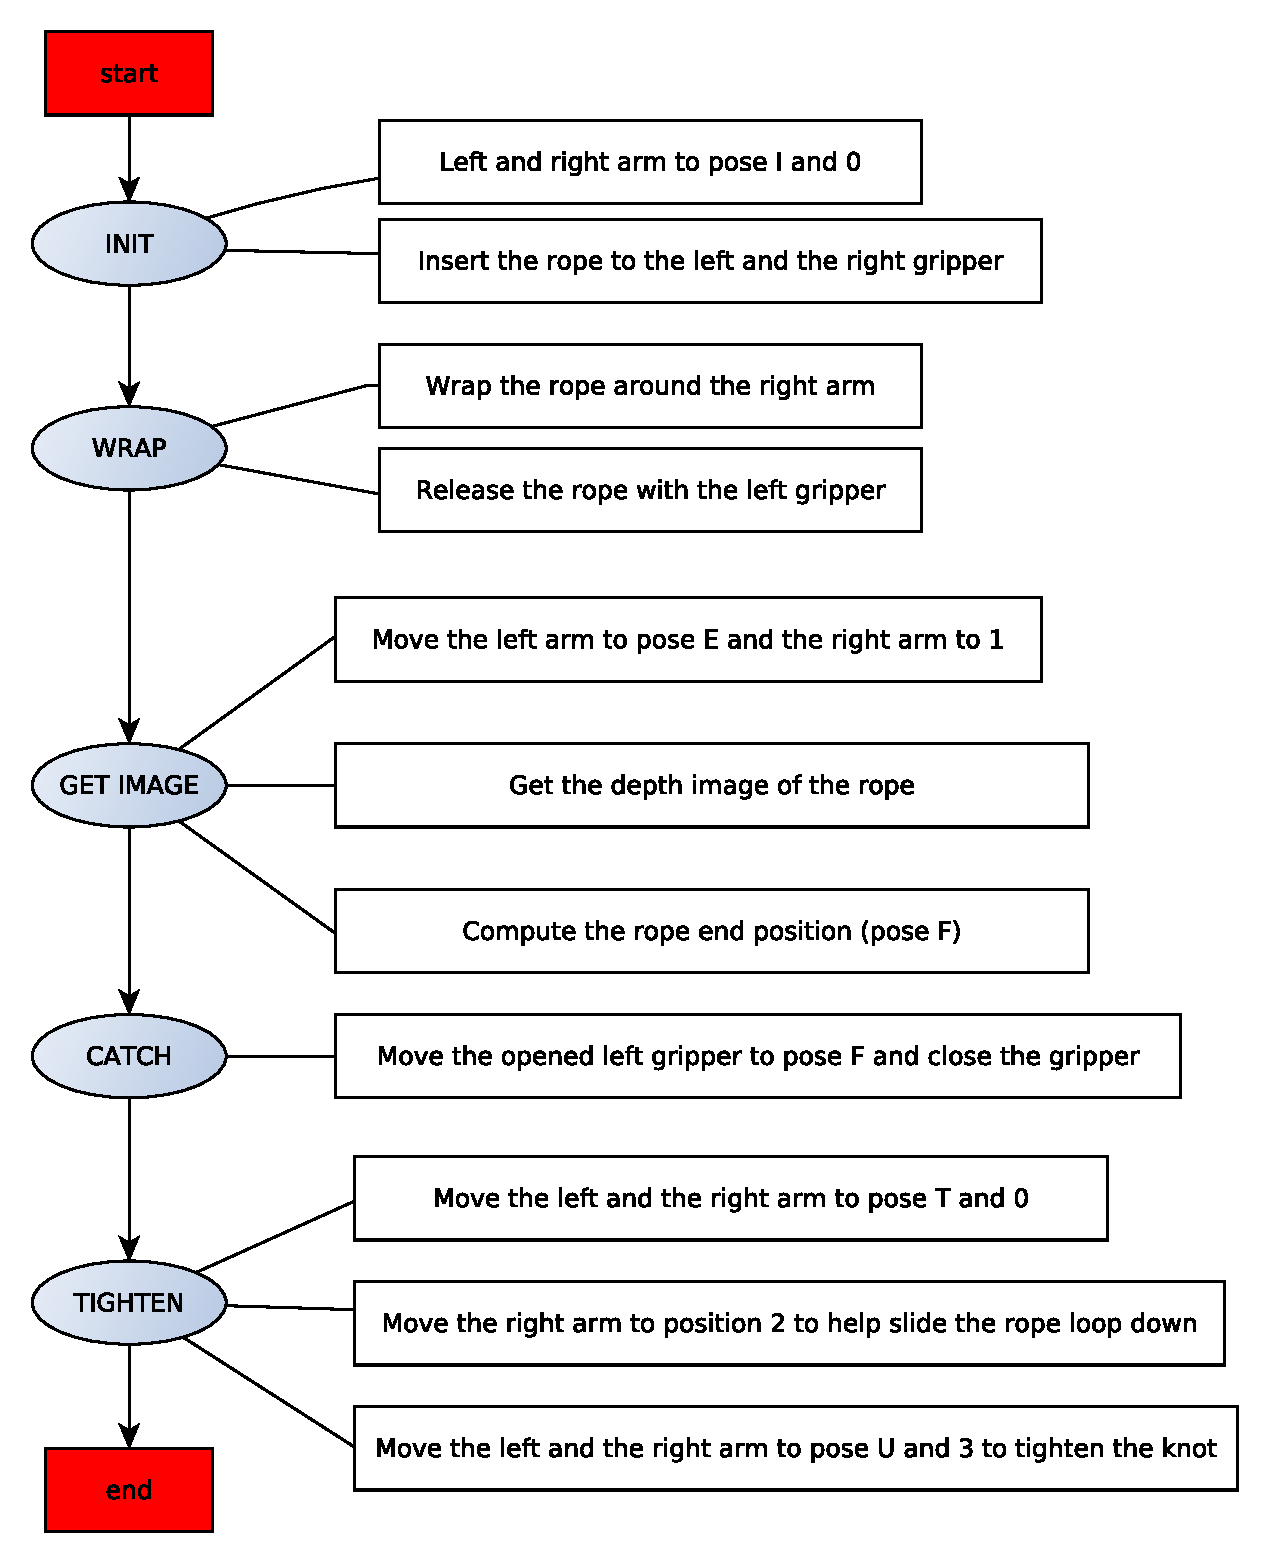
\includegraphics[width=0.8\textwidth]{TyerWorkflow.pdf}
        \centering
        \caption{Knot-tying work-flow.}
        \label{fig:TyerWorkflow}
        \end{figure}

        \begin{figure}
            \centering
            \begin{tabular}{c|c}
            \includegraphics[width=0.4\textwidth]{01Init.png}
            &
            \includegraphics[width=0.4\textwidth]{02Wrap.png} \\
            1 & 2 \\
            \hline
            \includegraphics[width=0.4\textwidth]{03GetImage.png}
            &
            \includegraphics[width=0.4\textwidth]{04Catch.png} \\
            3 & 4 \\

            \end{tabular}
            \caption{1: INIT, 2: WRAP, 3: GET IMAGE, 4: CATCH.}
            \label{fig:TyerStates}
        \end{figure}


        \begin{figure}
        \includegraphics[width=0.6\textwidth]{05Tighten.png}
        \centering
        \caption{TIGHTEN.}
        \label{fig:TyerTighten}
        \end{figure}



        \paragraph{INIT}~\\
        \noindent The tying procedure starts with the two grippers facing each other, right in pose $P_I$ and left in $P_0$ (see Figure~\ref{fig:TyerStates} - 1). Both grippers hold the ends of the rope.

        \paragraph{WRAP}~\\
        \noindent The right arm goes through poses $P_A$, $P_B$, $P_C$ and $P_D$ (see Figure~\ref{fig:TyerStates} - 2). The rope thus forms a loop around the left arm. Finally, the right gripper releases the rope end.

        \paragraph{CAPTURING THE IMAGE}~\\
        First, the left arm turns to pose $P_1$ to enable catching the rope end later. Second, the right arm moves to pose $P_E$ in order to have a good view of the rope loop and the rope end hanging on the left arm (see Figure~\ref{fig:TyerStates} - 3). Third, the right gripper closes and moves to get out of sight. The point cloud from the Kinect sensor is captured. Finally, the rope end is detected from the depth image. Pose of the rope end $P_F$ is computed.

        \paragraph{CATCH}~\\
        \noindent  The right gripper opens, the right arm moves to pose $P_F$ to catch the rope end. The gripper closes again. Next, the right arm moves back out of the loop to pose $P_G$ (see Figure~\ref{fig:TyerStates} - 4).

        \paragraph{TIGHTEN}~\\
        \noindent After the rope end is caught, both arms move to poses $P_T$ and $P_0$. The left arm then moves to pose $P_2$ to help the rope loop slide down of the robot arm . Finally, both arms start slowly moving from each other to poses $P_U$ and $P_3$ (see Figure~\ref{fig:TyerTighten}). The magnitude of the $z$-coordinate of the force from the right force sensor $F_z$ is measured. If the measured force exceeds the experimentally estimated threshold $F_{thresh} = \SI{10}{N}$ (meaning that the knot is already tightened), the motion of both arms is stopped.


    \section{Experiments}
        I tested the developed knot-tying script on ropes R1-5 (see Table~\ref{table:AvailableRopes}). Since R6 is flat and thus it is hard to detect it in the depth image, it was omitted from the experiments.

        I also changed the width parameter $w$ to 10. I did it due to further experiments with the red rope. Sometimes the rope end and rope loop were very close to each other. If $w=15$, both connected components merged into one and the rope end detection was not possible.

       The observations are listed below:
%
        \begin{itemize}\itemsep 0pt
            \item The proposed solution was successful in the case of R1 and R4 (successful rope end detection in Figure~\ref{fig:R4success}). It took around $65$ seconds to tie the knot (see video \textit{KnotTying.mpg} that can be found on the attached CD). Figure~\ref{fig:R1R4KnotTightening}, left side shows the knot tying process of R1 and Figure~\ref{fig:R1R4KnotTightening}, right side shows the successfully made knot on the rope R4.

            \begin{figure}
                \centering
                \begin{tabular}{cc}
                \includegraphics[height=0.3\textwidth]{R1KnotTightening.png}
                &
                \includegraphics[height=0.3\textwidth]{R4KnotTightening.png}

                \end{tabular}
                \caption{Left: Tightening the knot on the rope R1, Right: The knot made on the rope R4.}
                \label{fig:R1R4KnotTightening}
            \end{figure}

            \item The rope end was sometimes not found correctly in the case of R2 and R3 (see Figure~\ref{fig:R2R3failure}).
            \item R5 got stuck on the left arm during tightening.
        \end{itemize}


        \begin{figure}
            \centering
            \begin{tabular}{cc}
            \includegraphics[width=0.39\textwidth]{R4SegmentationAdj.png}
            &
            \includegraphics[width=0.39\textwidth]{R4RopeEndFoundAdj.png}

            \end{tabular}
            \caption{Left: R4 segmentation, Right: R4 rope end found.}
            \label{fig:R4success}
        \end{figure}

        \begin{figure}
            \centering
            \begin{tabular}{cc}
            \includegraphics[width=0.39\textwidth]{R2SegmentationAdj.png}
            &
            \includegraphics[width=0.39\textwidth]{R3SegmentationAdj.png}


            \end{tabular}
            \caption{Left: R2 segmentation, Right: R3 segmentation.}
            \label{fig:R2R3failure}
        \end{figure}

    \section{Discussion}
        It turned out that the proposed solution is mainly successful for non-white and non-twisted ropes. The rope should not be flat, but should also not be thicker than the gripper pitch.

        If the rope is white, the obtained segmentation in the depth image has huge gaps between the many connected components (see Figure~\ref{fig:R2R3failure}). Thus, the precondition that the segmentation should contain only two connected components is violated and the rope end detection fails.

        The twisted ropes not only cause the same problems during rope end detection as the white ones, but they also tend to get stuck on the robot arm.

        The mentioned issues relate to image segmentation. I used a simple segmentation algorithm because the image segmentation is an unsolved problem. Image segmentation is the object of the intensive research by others.



% Ribbon
\graphicspath{{Img/ribbon/}}

\chapter{Ribbon manipulation}

    \section{Assignment}
        The manipulation with the rhythmic gymnastics ribbon was chosen to demonstrate the dynamic motion combined with the visual/tactile perception on the \CloPeMa\/ robotic testbed.

        A common task for a human rhythmic gymnast is to swing the metallic pole hanging on a ribbon with one hand and catch it with the other hand (see Figure~\ref{fig:HumanGymnast}, the left side). Another rhythmic gymnast task is fast back and forth movements causing the ribbon to form spirals and other shapes that are nice to watch (see Figure~\ref{fig:HumanGymnast}, the right side).

        \begin{figure}[h]
            \centering
            \begin{tabular}{ccc}
            \includegraphics[height=0.35\textwidth]{HumanGymnastPendulum.png}
            %
            & &
            %
            \includegraphics[height=0.35\textwidth]{HumanGymnastShapes.png}
            \end{tabular}
            \caption{Left: Rhythmic gymnast catches the pole. Right: Rhythmic gymnast swings the ribbon.}
            \label{fig:HumanGymnast}
        \end{figure}



       \CloPeMa\/ ``robot rhythmic gymnast'' should perform a similar scenario that is defined to be the following. It starts from the state, in which the robot holds the pole hanging on the ribbon in its left gripper.
%
       \begin{enumerate}\itemsep0pt
       \label{enu:InformalAssignment}
            \item Swing the left arm in a way that the pole and the ribbon start to swing as well.
            \item Grasp the pole with the right gripper using one of the sensors present in the gripper.
            \item Make sure the pole was grasped, is held properly and release the ribbon from the left gripper.
            \item Perform a few fast moves with the right arm so that the ribbon forms a certain shape nice to watch.
       \end{enumerate}


    \section{Analysis}
        In order to fulfill the proposed scenario given in Section~\ref{enu:InformalAssignment}, I had to check a few capabilities of the \CloPeMa\/ robot.

        \subsection{Available sensors in the gripper}
            The gripper contains tactile, light, magnetic and proximity sensor in its tip $T$ \cite{SalanskyGripper}.

            \begin{figure}[h]
            \includegraphics[width=0.3\textwidth]{GripperDesc.png}
            \centering
            \caption{Gripper description.}
            \label{fig:GripperDesc}
            \end{figure}

        \subsection{Verifying the ability to catch the swinging pole}

            I decided to use the light sensor to detect the swinging pole. The output of the light sensor, the relative intensity $h$, goes up as the pole approaches it. If the pole swings with the gripper positioned at the turning point of the swinging motion, two peaks appear at the output of the light sensor. The first one appears when the pole passes the tip $T$ of the gripper on its way inside and the second one on its way out (see Figure~\ref{fig:GripperDesc}). The threshold for detecting the pole was set to $h = 30$. The time between the two peaks was measured. Figure~\ref{fig:SwingMeasurement} shows the obtained results. The total time during which the pole was inside the gripper was estimated to be $t_p = \SI{520}{ms}$.


            \begin{figure}[h]
            \includegraphics[width=0.5\textwidth]{SwingMeasurement.png}
            \centering
            \caption{Swinging pole detection.}
            \label{fig:SwingMeasurement}
            \end{figure}

        \subsection{Gripper closing speed}
            In order to catch a swinging pole on a ribbon, the capabilities of the gripper have to be explored.

            To control how much the gripper opens, parameter $n$ is introduced. It controls the gripper on a percentage like basis: $n=100$ for a fully closed gripper and $n=0$ for a fully opened gripper.

            The gripper was set to maximum speed (gripper frequency was set to $f_g = 25,000$) and the times $t_c$ (worst-case) the gripper needs to open and close were measured. The results are shown in Table~\ref{table:GripperClosingSpeeds}.

            \begin{table}\centering
            \ra{1.3}
            \begin{tabular}{@{}ccc@{}}\toprule
            Gripper state & $n$ & $ t_{c}$ [ms] \\ \midrule
            full open & 0 & 600 \\
            full close & 100 & 850 \\
            half close & 50 & 420 \\
            \bottomrule
            \end{tabular}
            \caption{Gripper speed.}
            \label{table:GripperClosingSpeeds}
            \end{table}

            To be able to catch the pole, the gripper cannot be fully opened as it cannot close fast enough. The gripper has to be only half opened to be able to catch the pole.

        \subsection{Maximal speed of the \CloPeMa\/ robot}
            The experiments performed to determine the maximum speed of the robot are described in~\cite{WagnerMaxRobotSpeed}. The robot can move faster if the executed trajectory has a low control point density.

            The \CloPeMa\/ testbed robot moves the fastest when it is operated directly through its control system on a trajectories taught in by a teach pendant. If the robot is managed by a program through ROS, its speed is limited to 20\% of its maximum speed at the level of the robot control system. For this reason, the following experiments were performed directly on trajectories taught in by the \CloPeMa\/ researcher Libor Wagner. Firstly, the robot had to perform a back and forth motion along a straight line in a general direction in 3D space (i.e. involving the motion of many robot joints simultaneously) at its maximum speed while holding the pole and the ribbon. The result was that the whole robot started shaking considerably due to the huge changes in acceleration. For this reason, for performing fast motions I decided to move the robotic arm using only one (and preferably the last) joint to reduce the motion impact on the whole construction.

            The conclusion is that the needed fast motions (to swing the pole and to make fast motions with the ribbon) will be performed using one joint only. In addition, to perform back and forth motions only the start and end point of the trajectory will be used to reduce the point density. The resulting motions are thus arcs.

    \section{Robotic rhythmic gymnast}
        \subsection{Equipment}
            I had a \SI{6}{m} long gymnastic ribbon (see Figure~\ref{fig:GymnasticRibbon}) and two gymnastic poles  at my disposal. The blue pole is shown in Figure~\ref{fig:GymnasticPoles}, left side  and the white pole in Figure~\ref{fig:GymnasticPoles}, right side. The properties (length $d$, weight $m$ and diameter $\phi$) of the gymnastic poles are shown in Table~\ref{table:PoleProperties}. The diameter $\phi$ is measured at the point where the pole is grasped by the right gripper.

            \begin{figure}[h]
            \includegraphics[width=0.5\textwidth]{RibbonAdj.png}
            \centering
            \caption{Rhythmic gymnastics ribbon.}
            \label{fig:GymnasticRibbon}
            \end{figure}

            \begin{figure}
                \centering
                \begin{tabular}{cc}
                \includegraphics[width=0.39\textwidth]{BluePoleAdj.png}
                %
                &
                %
                \includegraphics[width=0.39\textwidth]{WhitePoleAdj.png}
                \end{tabular}
                \caption{Left: Blue rhythmic gymnastics pole. Right: White rhythmic gymnastics pole.}
                \label{fig:GymnasticPoles}
            \end{figure}


            \begin{table}[h]\centering
            \ra{1.3}
            \begin{tabular}{@{}cccc@{}}\toprule
            Pole & Length $d$ [cm] & Weight $m$ [g] & diameter $\phi$ [mm] \\ \midrule
            blue & 59 & 29 & 0.84\\
            white & 57 & 22 & 0.72\\

            \bottomrule
            \end{tabular}
            \caption{Properties of the rhythmic gymnastics poles.}
            \label{table:PoleProperties}
            \end{table}


        \subsection{Experimental setup}
            The system consists of the end of the robot arm (left one), the ribbon and the pole (see Figure~\ref{fig:PoleInit}).

            Based on the given assignment in Section~\ref{enu:InformalAssignment} I designed a flow chart (see Figure~\ref{fig:Workflow}). It is explained below. I estimated the swinging angles $\alpha$ and $\theta$, catching threshold $h_{catch}$ and recatching threshold $r_{recatch}$ experimentally.

            The swinging angle $\alpha$ and $\theta$ are defined according to Figure~\ref{fig:SwingingAngle}.

            \begin{figure}[h]
            \includegraphics[width=0.2\textwidth]{SwingingAngleDef.png}
            \centering
            \caption{Definition of the swinging angles $\alpha$ and $\theta$.}
            \label{fig:SwingingAngle}
            \end{figure}

            \begin{figure}
            \includegraphics[width=0.9\textwidth]{PendulumWorkflow.pdf}
            \centering
            \caption{Robotic rhythmic gymnast workflow.}
            \label{fig:Workflow}
            \end{figure}

            \begin{figure}
                \centering
                \begin{tabular}{cc}
                \includegraphics[width=0.39\textwidth]{CaughtInsideAdj.png}
                %
                &
                %
                \includegraphics[width=0.39\textwidth]{CaughtWellAdj.png}
                \end{tabular}
                \caption{Left: The pole caught inside the gripper. Right: The pole caught well.}
                \label{fig:PoleCatching}
            \end{figure}

            \paragraph{INITIAL POSITION}~\\
                \noindent The right gripper holds the ribbon and the pole. The left arm is in the catching position. It means the right gripper should be positioned in the same plane in which the ribbon and pole swing. The turning point of the swinging motion should lie inside the gripper. It means that the pole should get inside the gripper at a certain point, but it should not hit the gripper.


            \paragraph{SWING THE RIBBON AND POLE}~\\
                \noindent The left robot arm swings back and forth between points $P_0$ and $P_1$ causing the pole and the ribbon to swing as well. The parameters $l = \SI{1}{m}$ and the swinging angle $\alpha = 22.5^o$ were used in experiments.

            \paragraph{CATCH THE POLE}~\\
                \noindent The right gripper starts closing from a half opened state as soon as the output of the light sensor exceed the closing threshold $h_{catch}=30$.

            \paragraph{Is the pole caught well?}~\\
                \noindent To determine whether the pole was caught inside the gripper (see Figure~\ref{fig:PoleCatching} Left) or caught well (see Figure~\ref{fig:PoleCatching} Right) the proximity sensor is used. If the recatching threshold exceeds $r_{recatch}= 5200$ an attempt to recatch the pole is made. It means that the gripper is opened for a short moment (to $n_{recatch}$) so that the pole moves towards its tip and closes back again ($n_{close}=100$) so that the pole stays inside the gripper.

            \paragraph{MOVE TO THE DANCING POSITION}~\\
                \noindent The left arm, which held the ribbon,  releases it and moves away. The right arm holding the pole moves up.

            \paragraph{SWING THE RIBBON}~\\
                \noindent The last joint of the right arm starts moving five times back and forth. The swinging angle is $\theta = 30.0^{o}$, so the total angle is two times bigger.


            \begin{figure}
            \includegraphics[height=0.4\textwidth]{PoleInit.png}
            \centering
            \caption{The hanging pole and the ribbon.}
            \label{fig:PoleInit}
            \end{figure}


        \subsection{Mathematical description of the swinging pole}

            My first idea was to describe the whole system mathematically as a double pendulum and then solve the appropriate differential equations. After that, I thought I would use the control theory to compute the motion of the left robot arm that will cause the maximum swinging amplitude of the pole hanging on the ribbon. However, after I finally came up with the system description using the Lagrange formalism, I realized that this approach is too complicated.

            For this reason, I tried to use the simplest description of a pendulum -- the mathematical pendulum (see Equation~\eqref{eq:MathematicalPendulum}).

            \begin{equation} \label{eq:MathematicalPendulum}
                \ddot{\varphi} = -\frac{g}{l}\sin(\varphi)
            \end{equation}

            The natural oscillations of a mathematical pendulum are described by Equation~\eqref{eq:T0}. In our case ($l = \SI{1}{m}$), $T_0 = \SI{2.01}{s}$.

            \begin{equation} \label{eq:T0}
                T_0 = 2 \pi \sqrt{\frac{l}{g}}
            \end{equation}

            I assumed that the swinging pole and ribbon resemble the mathematical pendulum (no damping, no air resistance, the whole mass concentrated only at the tip of the pendulum as a point mass, only small angle oscillations etc.). Thus, to achieve resonance and hence a maximal amplitude of the forced oscillations, the driving period of the robotic arm $T_r$ has to equal $T_0$.


        \subsection{Experiments}
            Based on the designed workflow (see Figure~\ref{fig:Workflow}), I made a video with two different gymnastic poles -- the white one and the blue one. It is called \textit{Gymnastics.mpg} and can be found on the attached CD. The end of the blue pole was wrapped in tape so that it is easier for a human to hold it and it was thicker than the end of the white pole.

            Although the swinging ribbon and the pole break almost all the assumptions connected with the mathematical pendulum, the experiments with the real swinging pole and ribbon show that the maximal amplitude increases as the period of the driving oscillations $T_r$ approaches $T_0$. Furthermore, the driving oscillations are applied in a way that the whole pendulum is swung by its end.

            Figure~\ref{fig:PoleCaught} shows the successful catching of the swinging white pole.

            \begin{figure}[h]
            \includegraphics[height=0.4\textwidth]{PoleCaught.png}
            \centering
            \caption{The white pole caught.}
            \label{fig:PoleCaught}
            \end{figure}



        \subsection{Discussion}
            The success rate of the pole catching depends on how the ribbon is held by the left arm. Since the gymnastic ribbon is \SI{6}{m} long it has to be folded so that the left gripper can hold it. However, the position of the plane in which the ribbon and pole will swing later greatly depends on how the gripper holds it. For this reason, the correct catching position of the right gripper has to be adjusted manually every time the ribbon is placed into the left gripper. However, once the catching position is properly adjusted, the success pole catching rate is > 90\%.

            In approximately 90\% of the cases the pole is caught inside the gripper and has to be recaught. In approximately 10\% of the cases the pole is caught well.

            The recatching parameter was determined experimentally. $n_{recatch\_white} = 80$ for the white pole and $n_{recatch\_blue} = 69$ for the blue pole (the thicker one). This parameter has to be set in advance by a human.

            The whole process runs fully automatically with the exception of setting $n_{recatch}$ and determining the correct catching position. The fact that I used two different poles of different thickness and weight shows the generality of the proposed solution.


\clearpage 

% Regrasping
\graphicspath{{Img/regrasping/}}

\section{Regrasping a rope}

    \subsection{Assignment}
        The last use case concerns regrasping a piece of a rope from one gripper to the other.

        The proposed scenario is the following.  It starts with the left gripper holding one end of the rope. The right gripper is open and is positioned towards the left gripper (see Figure~\ref{fig:RegraspInit}).
%
        \begin{enumerate}\itemsep0pt
            \item The left arm starts to move towards the right gripper.
            \item When the presence of the rope is detected inside the right gripper, the motion of the left arm is stopped.
            \item The right gripper closes, thus holding the other end of the rope.
            \item The left gripper opens and releases the rope.
            \item The left arm moves back and the functions of both arms are swapped.
            \item The whole procedure is repeated again. The right arm now moves towards the left one that catches the rope.
        \end{enumerate}

        \begin{figure}[h]
        \includegraphics[width=0.5\textwidth]{RegraspInit.png}
        \centering
        \caption{The initial position for regrasping the rope.}
        \label{fig:RegraspInit}
        \end{figure}

    \subsection{Regrasping workflow}
        In the following text, I use the definition of points shown in Figure~\ref{fig:GraspPoses} (front view). Points $P_{a,b,c}$ are connected with the left arm, while points $P_{1,2,3}$ are connected with the right arm. Point $P_0$ is used as the default point from which the rest of the points is calculated using the parameters $l$ and $h$, $l$ denotes the distance between the grippers and $h$ the length of the rope.

        \begin{figure}[h]
        \includegraphics[width=0.5\textwidth]{GraspPoses.pdf}
        \centering
        \caption{Defining the points.}
        \label{fig:GraspPoses}
        \end{figure}

        Based on the assignment, I designed the rope regrasping workflow that is shown in Figure~\ref{fig:RegraspingWorkflow}. The states of the procedure are shown in Figure~\ref{fig:RegraspingProcedure} and are described below.

        \begin{figure}
        \includegraphics[width=1.0\textwidth]{RegraspingWorkflow.pdf}
        \centering
        \caption{The regrasping workflow.}
        \label{fig:RegraspingWorkflow}
        \end{figure}


        \begin{figure}
            \centering
            \begin{tabular}{c|c}
            \includegraphics[width=0.4\textwidth]{GraspLeft.pdf}
            %
            &
            %
            \includegraphics[width=0.4\textwidth]{SwitchLeft.pdf}
            \\
            1 & 2 \\
            \hline
            \includegraphics[width=0.4\textwidth]{GraspRight.pdf}
            %
            &
            %
            \includegraphics[width=0.4\textwidth]{SwitchRight.pdf} \\
            3 & 4 \\

            \end{tabular}
            \caption{1: Grasp left, 2: Switch arms left, 3: Grasp right, 4: Switch arms right.}
            \label{fig:RegraspingProcedure}
        \end{figure}

        \paragraph{GRASP INIT}~\\
            The left arm moves to point~$P_a$ and the right one to point~$P_3$. The right gripper holds the rope that is hanging down freely. The left gripper is fully opened and is positioned in such a way that the rope that is going to be moved towards it in the next step will enter the inside of the gripper (see Figure~\ref{fig:RegraspingProcedure},~1).

        \paragraph{GRASP LEFT}~\\
            The left arm starts moving slowly towards point~$P_b$. The rope thus enters the right gripper. As soon as the rope is detected (see Section~\ref{sec:DetectingTheRope}), the movement of the left arm is stopped and the right gripper closes, thus catching the rope (see Figure~\ref{fig:RegraspingProcedure}, 1).

        \paragraph{SWITCH ARMS LEFT}~\\
            First, the left gripper releases the upper end of the rope. It falls down, now hanging just from the right gripper. Second, the left arm moves to point~$P_c$ thus reaching a pose in which it will later be able to catch the moving rope. Finally, the right gripper turns by \SI{180}{\degree} to unwrap the rope from the gripper (see Figure~\ref{fig:RegraspingProcedure}, 2).

        \paragraph{GRASP RIGHT}~\\
            See \textbf{GRASP LEFT}, the function of both arms is swapped (see Figure~\ref{fig:RegraspingProcedure}, 3).

        \paragraph{SWITCH ARMS RIGHT}~\\
            See \textbf{SWITCH ARMS LEFT}, the function of both arms is swapped (see Figure~\ref{fig:RegraspingProcedure}, 4).

        The gripper rotates \SI{180}{\degree} around the $x$-axis upon transition from points $P_3$ to $P_1$ in the case of the right gripper and from $P_C$ to $P_A$ in the case of the left gripper. Let us know examine the case of the right gripper. The rope end that has fallen down from the left gripper might now be a bit ``wrapped'' around the right gripper (see Figure~\ref{fig:WrappedRopeCloseUp}). Therefore, the right gripper has to rotate to ensure that the rope gets ``unwrapped'' and can hang down freely.

        \begin{figure}[h]
        \includegraphics[width=0.3\textwidth]{WrappedRopeCloseUp.png}
        \centering
        \caption{The rope wrapped around the gripper.}
        \label{fig:WrappedRopeCloseUp}
        \end{figure}


    \subsection{Detecting the rope in the gripper} \label{sec:DetectingTheRope}

        The rope detection algorithm was originally tested on the rope R2 (white and twisted rope, see Table~\ref{table:AvailableRopes}). The left gripper holding the R2 rope was moved to point $P_b$ and the output of the proximity and light sensor placed in the right gripper was measured.

        I decided to use the proximity sensor over the light sensor for the rope detection, because the peak in the output of the proximity sensor was more distinct than the peak in the output of the light sensor (see Figure~\ref{fig:RopeDetection}, left side).

        The motion of the arm holding the rope is stopped, when a peak in the output of the proximity sensor passes. This approach proves more robust for ropes of different thicknesses (a thicker rope produces a higher peak) than a simple thresholding. However, a threshold is used to detect the rise of the peak. Initially, I set up the threshold to $r_0 = 100$ (see Figure~\ref{fig:RopeDetection}, right side). The threshold $r_0$ makes sure that the rope detection process does not react on noise in the output of the proximity sensor.


        \begin{figure}[h]
            \centering
            \begin{tabular}{cc}
            \includegraphics[width=0.49\textwidth]{ProximityVsLight.png}
            %
            &
            %
            \includegraphics[width=0.49\textwidth]{ProximityPeak.png}
            \end{tabular}
            \caption{Left: Comparing the proximity and light sensor. Right: Detecting the peak.}
            \label{fig:RopeDetection}
        \end{figure}


    \subsection{Experiments}
        I found out that the rope R2 is not suitable for the regrasping procedure. It did not become straight after it was regrasped, it was rather bent to one side. This behavior prevents the successful consecutive regrasping. For this reason, I decided to use a different rope (see Figure~\ref{fig:Regrasping}). To ensure that it becomes straight again, it has a weight on each end.

        I did not have to change the rope detection algorithm, it worked well for a thinner rope also. The only thing I had to adjust was to lower the threshold $r_0$ to 20, since the peak in the output of the proximity sensor became smaller.

        \begin{figure}
        \includegraphics[width=0.5\textwidth]{Regrasping.png}
        \centering
        \caption{The left arm regrasps the rope.}
        \label{fig:Regrasping}
        \end{figure}

        The procedure ran successfully for regrasping the rope from the right gripper to the left and back. It took \SI{34}{s}. The experiment was recorder on video that is called \textit{RegraspRope.mpg} and can be found on the attached CD.

    \subsection{Discussion}
        Although the robot managed to regrasp the rope successfully, a few additional features would have to be implemented in order to make the process continuous (i.e. to be able to regrasp the rope many times in a row). The point in which the upper gripper releases the rope should be moved a bit to the side. In this way, the rope would fall to a predictable side of the lower gripper. Thus, it would be possible to always unwrap the rope from the gripper by turning it by \SI{180}{\degree}. This does not happen in the present case, since the rope is released directly above the gripper and thus it is not predictable on which side of the gripper it falls down. 

% Implementation
\graphicspath{{Img/implementation/}}
\section{Implementation}
     I programmed all the needed scripts and algorithms in Python 2.7.3 \cite{Python}. The communication with the various installed sensors was done through \emph{Robotic Operating System} (ROS) \cite{ROS2009}. I used the \emph{Moveit!} package to control the movements of the robot \cite{moveit}.

    \subsection{How to run the code}
        The following manual is applicable for the PC's at the \CloPeMa\/ laboratory. The required operating system is Ubuntu 12.04 with installed ROS Hydro.

        To launch the \CloPeMa\/ Rviz 3D Visualization Tool~\ref{fig:rviz}, run the following code in the console.

        \begin{lstlisting}[language=bash, label={lst:StartClopema}]
roscore
roslaunch clopema_launch start_robot.launch
        \end{lstlisting}

        \begin{figure}[h]
        \includegraphics[width=0.5\textwidth]{rviz.png}
        \centering
        \caption{Rviz 3D Visualization Tool.}
        \label{fig:rviz}
        \end{figure}


        There is a Moveit! plugin, so one can move the robotic arms simply by dragging them in the visualization.

        The code that I wrote can be found in the \textit{clopema\_compliance\_2} package. Type the following to the console to navigate to the corresponding folder.
                \begin{lstlisting}[language=bash, numbers=none]
roscd clopema_compliance_2
                \end{lstlisting}


        The main code for the four tasks consists of four classes each placed in a separate module (class Shooter in shooter2.py for the slingshot, Tyer in tyer2.py for the knot-tying, Pendulum in pendulum2.py for the rhythmic gymnastics and Regrasper in regrasper.py for the regrasping). Each file contains a main() method that starts the main sequence for that particular module. I prepared the so called launch files that are used not only to start the main method, but also to launch all the required sensors. They are called \textit{shooter.launch}, \textit{tyer.launch}, \textit{pendulum.launch} and \textit{regrasper.launch}. To run the launch file, type:

                \begin{lstlisting}[language=bash, numbers=none]
roslaunch clopema_compliance_2 *.launch
                \end{lstlisting}

        If you wish to inspect and run the different methods of the classes separately, use the \textit{IPython} console. There are four test files that only initialize an instance of that particular class. One can then run the different methods one by one. The following code is an example for the \textit{Regrasper} class.


                \begin{lstlisting}[language=bash, numbers=none]
# First navigate to the corresponding folder.
ipython # Start the IPython console.

# Initialize an instance of Regrasper class.
run regrasper2_test.py

# Then run the different methods individually, for example:
r.init() # The robot moves to the initial position.
r.insert_rope_left() # Insert the rope to the left gripper.
r.grasp_left() # Regrasp the rope.
                \end{lstlisting}

        Note that you will have to start all the required sensors manually.

              \begin{lstlisting}[language=bash, numbers=none]
roslaunch clopema_launch force_sensors.launch # Start both force sensors.
roslaunch clopema_launch xtion1.laucnh # Start the xtion sensor in the r1 arm.
                \end{lstlisting}

        The documentation for all four modules can be found in the Use Cases Reference in Appendix~\ref{sec:appendix} or on the attached CD.



    \subsection{Description of the developed reusable code}
        I successfully implemented a few classes (I call them managers) in Python that simplify the work with the \CloPeMa\/ robot and that are made to be used by others as well. These classes build on top of the \CloPeMa\/ testbed and provide more advanced functionality.

        \emph{MoveManager} covers many areas that are connected with controlling the movements of the robot arms. There are functions available for moving the arm along a straight line and for turning only one joint. Furthermore, there are functions that enable computing distance between the different coordinate systems of the robot and for transforming poses using the axis-angle notation.

        \emph{GripperManager} covers the operation of the robot gripper. One can set its closing speed. Not only can one open and close the gripper fully, but there are functions that enable partial opening as well.

        \emph{ForceManager} provides the functionality connected with the force sensor. One can stop the motion of the robot arm or open/close the gripper, if the measured force exceeds a certain threshold.

        \emph{CameraManager} provides the functionality connected with the Kinect sensor. There are function to obtain either the RGB or depth image of the scene. The algorithm for finding connected components is implemented in this module.

        \emph{ProximityManager} provides functions connected with the light and proximity sensors that are placed in the grippers. It can be used for closing the gripper, if the output of the light or proximity sensor exceeds a certain threshold.

        I also generated a documentation that contains the most used methods as well as a short description of the developed modules. Below is an excerpt taken from the automatically generated documentation describing the managers. The detailed description for the developed methods and classes can be found in the Manager Reference in Appendix~\ref{sec:appendix}. The full generated documentation in pdf and in HTML can be found on the attached CD.

        

    \includepdf[pages={5-6}]{Src/clopema_compliance.pdf}


% Conclusions
\section{Conclusions}
    In the course of working on the master thesis, I implemented four use case scenarios. The feedback from the various sensors of the two arm \CloPeMa\/ robot is used to accomplish tasks that involve perception and manipulation with soft objects.    

    \subsection{Slingshot}

        \begin{figure}[h]
            \centering
            \begin{tabular}{cc}
            \includegraphics[height=0.3\textwidth]{Img/slingshot/attached_slingshotAdj.png}
            %
            &
            %
            \includegraphics[height=0.3\textwidth]{Img/slingshot/attached_flat_slingshot.png}
            \end{tabular}
            \caption{Left: The traditional slingshot. Right: The flat slingshot.}
            \label{fig:Slingshots}
        \end{figure}

        I designed two slingshots to shoot from -- the so called traditional slingshot (see Figure~\ref{fig:Slingshots}, left side) and the flat slingshot (see Figure~\ref{fig:Slingshots}, right side). Both had to be attached directly to the robot arm. Since the design of the grippers have changed, it was not possible to attach the elastic string directly to it as the projectile could damage some of the sensors placed in the gripper.

        I developed a fully automated shooting procedure that includes loading the projectile, stretching the elastic string to a specified force and adjusting the shooting angle. Thus, a few shots with the same parameters could be shot in a row. The force feedback was used.

        \begin{figure}[h]
        \includegraphics[width=0.5\textwidth]{Img/conclusion/HitTargetAdj.png}
        \centering
        \caption{The projectile hits the target.}
        \label{fig:HitTarget}
        \end{figure}

        I made a few experiments with both slingshots. It involved shooting on a target hanging on the wall and measuring the height, at which the projectile hit the wall. I compared the experimental results with the theoretically calculated values. In case of the traditional slingshot, the results differed a lot. I think it was mainly due to the fact that it was not possible to attach the traditional slingshot tightly to the robot arm. Another reason is for instance the fact that even a small uncertainty in one of the parameters (e.g. the weight of the projectile) influences the theoretical calculation to a high degree. The results concerning the flat slingshot were significantly closer to the theoretical values than in the previous case, yet still not perfect. In order to improve the results, the way the shooting angle is adjusted would have to change.

        Despite the issues stated above, I was able to repeatedly hit the target hanging on the wall (see Figure~\ref{fig:HitTarget}). The success rate was around 50\% for the traditional slingshot and above 90\% for the flat slingshot. I made a video called \textit{TraditionalSlingshot.mpg} featuring the traditional slingshot that shows the whole shooting procedure. It can be found on the attached CD.

        Further work could involve connecting the shooting procedure with an automatic target recognition using for instance the Kinect sensor. The parameters of the shooting such as the shooting angle and the force with which the projectile is shot would then be computed automatically so that the projectile hits the target. In order to achieve such functionality, the slingshot would have to be redesigned further. For instance, the elastic string should be made of a different material so that the force changes gradually with its stretch and not sharply as it is the case of the present elastic string.


    \subsection{Knot-tying}
        I successfully implemented a fully automated knot-tying procedure. I tested the proposed knot-tying sequence on two persons (see Figure~\ref{fig:ABExamples}); one that sees normally (subject A) and one that is blind (subject B). I made conclusions for the robotic knot-tying based on the observed behavior of the two subjects. I especially focused on the blind subject, because his movements resemble in a way the movements of the  \CloPeMa\/ robot more closely than the movements of the normally seeing subject.

        \begin{figure}[h]
            \centering
            \begin{tabular}{cc}
            \includegraphics[height=0.3\textwidth]{Img/tyer/ATwoFingers.png}
            %
            &
            %
            \includegraphics[height=0.3\textwidth]{Img/tyer/BLookingForRopeEnd.png}
            \end{tabular}
            \caption{Left: Subject A holds the rope with 2 fingers. Right: Subject B caught the rope end.}
            \label{fig:ABExamples}
        \end{figure}

        I implemented a procedure that finds the rope end in an image using the connected components algorithm (see Algorithm~\ref{alg:ConnectedComponents}). The rope end is found in the depth image, which makes the whole procedure invariant to the color of the rope. However, the rope segmentation from the depth image is prone to errors if the rope is twisted and shiny (see Section~\ref{sec:AvailableRopes}. Two example images from a successful knot-tying are shown in Figure~\ref{fig:R1R4ExampleImgs}.

        \begin{figure}[h]
            \centering
            \begin{tabular}{cc}
            \includegraphics[height=0.3\textwidth]{Img/tyer/R1KnotTightening.png}
            &
            \includegraphics[height=0.3\textwidth]{Img/tyer/R4KnotTightening.png}

            \end{tabular}
            \caption{Left: Tightening the knot on the rope R1, Right: The knot made on the rope R4.}
            \label{fig:R1R4ExampleImgs}
        \end{figure}

        Moreover, I used the feedback from the force sensor to determine that the knot has been already tightened. In that case, further stretching of the rope is stopped.

        Further work could focus on making the rope end detection better. First, the code involving image processing could be made faster by for instance rewriting the Python code into \Cplusplus. Second, the information about the color of the rope could be combined with the depth information to improve the rope segmentation procedure. In addition, further work could focus on distinguishing the case when the rope end was successfully caught from the case when it was not. The finding of the rope end and the catching of it could be then repeated if necessary.

    \subsection{Ribbon manipulation}
        Based on the observation of a human rhythmic gymnast, I developed a procedure that allows the \CloPeMa\/ robot to catch a swinging pole hanging on a ribbon. The task involves mathematical modeling of the swinging pole and ribbon and exploring the capabilities of the gripper such as its maximum closing speed. The light and proximity sensors placed in the robot gripper were used to detect the presence of the pole and to determine whether the pole was caught well or not. Figure~\ref{fig:HumanAndRobotGymnastPoleCatch}, left side shows the human rhythmic gymnast that caught a swinging pole and Figure~\ref{fig:HumanAndRobotGymnastPoleCatch}, right side shows the \CloPeMa\/ robot performing the same.

        \begin{figure}[h]
            \centering
            \begin{tabular}{cc}
            \includegraphics[height=0.39\textwidth]{Img/ribbon/HumanGymnastPendulum.png}
            %
            &
            %
            \includegraphics[height=0.39\textwidth]{Img/ribbon/PoleCaught.png}
            \end{tabular}
            \caption{Left: The human rhythmic gymnast catching a swinging pole. Right: The robotic gymnast catching a swinging pole.}
            \label{fig:HumanAndRobotGymnastPoleCatch}
        \end{figure}

        I also investigated the possibilities of performing fast motions with the \CloPeMa\/ robot. The aim was to mimic a human rhythmic gymnast performing fast motions with the ribbon (see Figure~\ref{fig:HumanAndRobotGymnastShapes}, left side) thus forming shapes that are nice to watch. Figure~\ref{fig:HumanAndRobotGymnastShapes}, right side shows the robotic counterpart doing the same.

        \begin{figure}[h]
            \centering
            \begin{tabular}{cc}
            \includegraphics[height=0.39\textwidth]{Img/ribbon/HumanGymnastShapes.png}
            %
            &
            %
            \includegraphics[height=0.39\textwidth]{Img/ribbon/RobotGymnastShapes.png}
            \end{tabular}
            \caption{Left: The human rhythmic gymnast performing fast motions with the ribbon. Right: Robotic gymnast performing fast motions with the ribbon.}
            \label{fig:HumanAndRobotGymnastShapes}
        \end{figure}

        However, the fact that the maximum speed of the robot is limited to 20\% when it is operated through ROS does not allow the ribbon to be swung fast enough to form a visually nice shape. The results obtained when operating the robot through a teach pendant (thus reaching the maximum robot speed) were better. Yet operating the robot at its maximum speed in an unskilled manner for longer periods of time might cause damage.

    \subsection{Regrasping a rope}
        I successfully designed a scenario in which the \CloPeMa\/ robot regrasps a rope from one gripper to the other and back. The procedure is fully automated. The proximity sensor is used to detect the presence of the rope in the gripper. To make the rope detection process more robust so that it can handle ropes of different thickness, the gripper closes when a peak in the output of the proximity sensor passes (I do not use a simple thresholding).

        The regrasping procedure was recorded in the video that is called \textit{RegraspRope.mpg} and can be found on the attached CD. I have also taken a few screen shots from the procedure to illustrate it better. They are shown in Figure~\ref{fig:RegraspingProcess}.

        \begin{figure}[h]
            \centering
            \begin{tabular}{c|c}
            \includegraphics[width=0.4\textwidth]{Img/regrasping/RegraspInit.png}
            &
            \includegraphics[width=0.4\textwidth]{Img/regrasping/Regrasping.png} \\
            1 & 2 \\
            \hline
            \includegraphics[width=0.4\textwidth]{Img/regrasping/RopeDownLeft.png}
            &
            \includegraphics[width=0.4\textwidth]{Img/regrasping/RegraspingRight.png} \\
            3 & 4 \\
            \hline
            \includegraphics[width=0.4\textwidth]{Img/regrasping/RopeDownRight.png}
            &
            \includegraphics[width=0.4\textwidth]{Img/regrasping/SwitchArmsRight.png} \\
            5 & 6 \\

            \end{tabular}
            \caption{1: The initial pose. 2: The rope caught with the right gripper. 3: The rope released from the left gripper. 4: The rope caught with the left gripper. 5: The rope released from the right gripper. 6: Back to the initial pose.}
            \label{fig:RegraspingProcess}
        \end{figure}

        Further work could improve the release of the rope. The present solution does not allow regrasping of the rope many times (see the difference between 1 and 6 in Figure~\ref{fig:RegraspingProcess}), since it is not sure on which side of the gripper the rope falls down. Therefore, it is not possible to ensure that the rope is unwrapped correctly. This issue can be solved by avoiding the release of the rope directly above the lower gripper. The rope should be released a bit to the side, so that it falls to a predictable side of the lower gripper.

    \subsection{Documentation of the developed code}
        I made a documentation of the code that I wrote. The full version in HTML (see screen-shot in Figure~\ref{fig:DocHTML}) and pdf can be found on the attached CD.

        \begin{figure}[h!]
        \includegraphics[width=0.5\textwidth]{Img/conclusion/DocHTML.png}
        \centering
        \caption{HTML documentation of the source code.}
        \label{fig:DocHTML}
        \end{figure}

        A part of the developed code are the so called managers. These are classes that simplify the work with the \CloPeMa\/ robot. \emph{MoveManager} and \emph{GripperManager} provide the functionality connected with the movement of the robot and its grippers. \emph{ForceManager}, \emph{CameraManager} and \emph{ProximityManager} encapsulate methods connected with the force/torque sensor, Kinect sensor and the light and proximity sensors in the grippers. These classes could be the entry point for somebody new who wants to start working with the robot.



\clearpage 

\bibliography{biblio}
\bibliographystyle{ieeetr}
\clearpage

% Appendix
%
\ctuAppendix{CD content} \label{sec:appendix}
    \begin{tabular}{rl}
    & \\[.5cm]
      \textit{ThesisTadeasLejsek.pdf} & The PDF version of this document.\\
        \textit{src/} & \LaTeX version of this document.\\       
        \textit{clopema\_compliance/} & ROS Package with the library source codes.\\
        \textit{doc/} & HTML and pdf documentation to the source code.\\         
        \textit{video/} & Selected videos from the experiments.\\
    \end{tabular}
    \clearpage

% \section*{Source code documentation}
    \includepdf[pages={7-14}]{Src/clopema_compliance.pdf}

\end{document} 